\documentclass[11pt,oneside,a4paper]{article}


% Usepackages
\usepackage[left=2cm,right=2cm,top=2cm,bottom=2cm]{geometry}
\usepackage[intoc]{nomencl}
\usepackage{float}
\usepackage{floatflt}
\restylefloat{figure}
\usepackage{color}
\usepackage{siunitx}
\usepackage[utf8]{inputenc}
\sisetup{separate-uncertainty}
\usepackage[T1]{fontenc}
\usepackage[english]{babel}
\usepackage{ae}
\usepackage{chngcntr}
\usepackage{natbib}
\usepackage[overload]{empheq}
\usepackage{amsthm}
\usepackage{amssymb}
\usepackage{latexsym}
\usepackage[title]{appendix}
\usepackage{multicol}
\usepackage{amsmath}
\usepackage{amsfonts}
\usepackage{tabularx}
\usepackage{caption}
\usepackage[multiple]{footmisc}
\usepackage{color}
\definecolor{grau}{rgb}{0.95,0.95,0.95}
\definecolor{dunkelgrau}{rgb}{0.8,0.8,0.8}
\usepackage{colortbl}
\usepackage{authblk}
\usepackage{url}
\usepackage{xcolor}
\usepackage{pgf}
\usepackage{wrapfig}
\usepackage[printwatermark]{xwatermark}
\usepackage{xcolor}
\usepackage{graphicx}
\usepackage{lipsum}
\usepackage{tikz}
\usepackage{abstract}
\numberwithin{equation}{section}
\usepackage{mathbbol}
\usepackage{amssymb}             % AMS Math
\usepackage[colorlinks=true,linkcolor=blue,urlcolor=blue]{hyperref}
\usepackage{multirow}
\usepackage{cases}
\usepackage{hhline}


\DeclareSymbolFontAlphabet{\amsmathbb}{AMSb}%






% Commands
\newcommand{\pa}{\partial}
\newcommand{\mr}[1]{\mathrm{#1}}
\newcommand{\mb}[1]{\mathbf{#1}}
\newcommand{\bo}[1]{\boldsymbol{#1}}
\newcommand{\fh}{f_\mr{h}^\mr{D}}
\newcommand{\fho}{f_\mr{h0}^\mr{D}}
\newcommand{\fhi}{f_\mr{h1}^\mr{D}}
\newcommand{\Bpa}{B_\parallel^\ast}
\newcommand{\intom}{\int_{\hat{\Omega}}}
\newcommand{\hatC}{\hat{\bo{C}}^1}


\renewcommand\Affilfont{\fontsize{10}{20}\itshape}

% Title
\title{MHD-kinetic hybrid code based on structure-preserving finite elements with 
particles-in-cell}

% Date
\date{}

% Authors and affiliations
\author[1,2,*]{Florian Holderied}
\author[1,3]{Stefan Possanner}
\author[1]{Xin Wang}

\affil[1]{\textit{Max Planck Institute for Plasma Physics, Boltzmannstrasse 2, 85748 Garching, 
Germany}}
\affil[2]{\textit{Technical University of Munich, Department of Physics, James-Franck-Strasse 1, 85748 Garching, Germany}}
\affil[3]{\textit{Technical University of Munich, Department of Mathematics, Boltzmannstrasse 3, 85748 Garching, Germany}}
\affil[*]{\textit{Corresponding author: Florian Holderied, florian.holderied@ipp.mpg.de}}





\begin{document} 

\maketitle

\begin{abstract}
\noindent 
We present a STRUcture-Preserving HYbrid code - STRUPHY - for the simulation of magneto-hydrodynamic (MHD) waves interacting with a population of energetic particles far from thermal equilibrium (kinetic species). The implemented model features linear, ideal MHD equations in curved, three-dimensional space, coupled nonlinearly to the full-orbit Vlasov equations via a current coupling scheme. The algorithm is based on finite element exterior calculus (FEEC) for MHD and particle-in-cell (PIC) methods for the kinetic part; it provably conserves mass, energy, and divergence-free magnetic field, irrespective of metric (= space curvature), mesh parameters and chosen order of the scheme. These properties enable reliable long-time simulations of energetic particle physics in complex geometries, covering the whole range of MHD waves. In STRUPHY, the finite element spaces are built from tensor products of univariate B-splines on the logical cuboid and can be made high-order by increasing the polynomial degree. Time-stepping is based on Poisson splitting with implicit sub-steps, mitigating CFL conditions from fast magneto-acoustic waves. High-order time splitting schemes can be used in this regard.  
\end{abstract}


\section{Introduction}
Plasma waves in magneto-hydrodynamic (MHD) fluids can be resonantly excited by energetic particles with thermal speeds in the range of the Alfv\'en velocity. Such 
wave-particle interactions are observed for instance in deuterium-tritium fusion reactors, where hot $\alpha$-particles can destabilize shear Alfv\'en modes and thus compromise confinement time \cite{Heidbrink_basics2008,Lauber2013,Chen_Zonca_review2016}. Another example is the interaction of energetic electrons in the solar wind with Whistler waves propagating in Earth's magnetosphere. This interaction can lead to new types of electromagnetic waves whose spectrograms show discrete elements with rising or falling frequencies with respect to time (also known as frequency chirping) \cite{Tsurutaniatal1974,Burtisetal1976,Santoliketal2004}. The associated nonlinear dynamics in realistic scenarios such as fusion reactors or solar wind can be studied via computer simulation of suitable model equations. The latter range from full kinetic models of all involved plasma species (bulk and energetic particles), over hybrid codes to reduced fluid simulations, all compared in a recent benchmark study \cite{Konies_benchmark2018}. The notion of a "hybrid code" implies the following two crucial features:
\begin{enumerate}
\item Use of reduced model equations for bulk plasma (for instance 
fluid instead of kinetic).
\item Fully self-consistent description of nonlinear dynamics (beyond the linear phase).
\end{enumerate}
Examples of successful implementations of hybrid codes in Fusion research are MEGA \cite{Todo_MEGA1998}, 
M3D-K \cite{Belova1997,Belova_M3D1999}, and HMGC \cite{Zonca_HMGC1995,XinWang2011}. The appeal of hybrid codes is three-fold: a) reduced numerical cost compared to fully kinetic simulations, b) inclusion of non-equilibrium dynamics (wave-particle resonances) compared to pure fluid simulations and c) possibility of direct comparison with analytic computations (for linear dynamics). The drawback is the increased complexity of model equations. For instance, while the geometric structure (ie. Poisson bracket and/or variational principle) of MHD equations has been 
known for decades \cite{MorrisonGreene1980}, the underlying structure of MHD-kinetic hybrid models has been discovered only very recently \cite{Tronci2010,Tronci2017}. This shows that the proper derivation of MHD-kinetic hybrids that respect fundamental physics principles such as energy conservation is a non-trivial task. As a consequence, little attention had been paid to these issues during the design of the first generation of hybrid codes mentioned above.

In parallel to the theoretical discoveries regarding hybrid models came the advent of geometric (or structure-preserving) methods for plasma equations, see \cite{Morrison2017} for a review. These methods obey many conservation properties implied by the geometric structure, such as conservation of energy, charge or momentum on the discrete level. The main idea is to discretize directly the underlying Poisson structure or variational principle, thus transferring geometric properties to a finite-dimensional setting. The very first structure-preserving geometric PIC algorithm was designed and implemented by Squire et al. in 2012 \cite{Squire2012}. Similar methods have later been successfully applied to Vlasov-Maxwell \cite{He_splitting2015,Qin2015,Xiao2017,Xiao2018}, Vlasov-Darwin \cite{Chacon2014} and Vlasov-Poisson equations \cite{Shadwick2013,Xiao_Qin2019}. The first structure-preserving geometric PIC algorithm using finite element exterior calculus (FEEC) was designed by He et al. in 2016 \cite{He_FEEC2016}. The same approach has later been taken by Kraus et al. \cite{GEMPIC2017} who used B-spline basis functions to efficiently build the discrete deRham complex, which contains N\'ed\'elec and 
Raviart-Thomas spaces. The theoretical foundation of FEEC has been laid by Arnold et al. \cite{ArnoldFalkWinther2006, ArnoldFalkWinther2010}; the interested reader may consult the recent book of Arnold \cite{Arnold_FEEC2018} for a comprehensive overview.  

In this work we apply the ideas of structure-preserving integration to a MHD-kinetic hybrid model, namely the Hamiltonian current-coupling (CC) scheme \cite{Tronci2010}. The equations consist of the three-dimensional, ideal MHD equations coupled to the collision-less, full-orbit Vlasov equation with three velocity degrees of freedom. The MHD part thus covers the entire set of MHD waves, namely shear Alfv\'en, slow- and fast magneto-acoustic waves. The kinetic equation contains the cyclotron motion of the energetic species, enabling the description of wave-particle resonances in this regime. The motivation for this work stems from the need of stable and reliable long-time simulations of energetic particle physics in tokamaks, stellarators and also space plasmas. In that regard, the version of STRUPHY presented in this paper can be viewed as the beginning of our quest to reach this goal by using the most modern numerical tools available, which ultimately will provide the necessary stability in nonlinear simulations. Future extensions of the code will feature also drift-kinetic or gyro-kinetic species, allowing for the efficient simulation of low-frequency phenomena.  
\color{black}

In the current version of the code, we linearize the MHD part and focus on the nonlinear coupling to the kinetic species, which acts back on the bulk plasma via charge and current densities (CC). FEEC is used for the discretization of the MHD part and PIC for the kinetic part. The concept is similar to the GEMPIC-approach in \cite{GEMPIC2017}, only that the role of the Maxwell equations is taken by the linear MHD equations. Another difference w.r.t. GEMPIC is that we discretize directly the equations rather than the variational principle or the Poisson bracket. There are three reasons for this: 1) linearized MHD equations lose their Hamiltonian structure if the magnetic background field is not chosen properly. In this case there is no such thing as a Poisson bracket or variational formulation, but our method of discretization still applies, 2) Poisson structures of extended hybrid models with two-fluid MHD, drift-kinetic or gyro-kinetic models are either not known or very cumbersome, such that pure "geometric" discretisation is not possible, and 3) we avoid a high level of abstraction in the presentation of the scheme. In fact, the mere existence of a Poisson structure on the continuous level is sufficient to translate several important conservation properties to the discrete level by applying FEEC to the equations directly. Our discretization of the CC hybrid models provably conserves energy, mass and the divergence-free magnetic field, irrespective of the metric, mesh parameters and chosen order of the scheme. This is thanks to the separation between topological and metric properties in the theory of differential forms, upon which FEEC is built, and due to the coupling with a particle-based kinetic solver. In STRUPHY, the FE spaces are built from tensor products of univariate B-splines of arbitrary order, either periodic or clamped, on the logical cuboid. Position space is expressed in logical coordinates, also for the kinetic species, during the entire simulation. Results in physical space are obtained in post-processing by a push-forward operation. The time stepping is implicit and based on Poison-splitting of a skew-symmetric matrix. Most of the sub-steps are solved via the Crank-Nicolson method (average vector-field). Lie-Trotter ans Strang splitting methods have been implemented, but higher-order methods would be in principle available \cite{McLachlanetal2012}.
\color{black}

This article is organized as follows. Section \ref{sec_model} first introduces the basic model equations, the MHD linearisation and the corresponding conservation laws. Model equations are presented in curvilinear coordinates and in terms of differential forms to prepare the application of FEEC. Based on this result, Section \ref{sec_discrete} describes in detail the spatial discretization, followed by a discussion of some properties of the resulting semi-discrete system of ordinary differential equations with continuous time variable. We also review the realization of the compatible finite element spaces along with projection operators on these spaces using B-spline basis functions, which are used in this work. Section \ref{sec_time} is devoted to the proposed time integration scheme based on Poisson splitting. Numerical results are shown in Section \ref{sec_experiments} before we summarize and conclude in Section \ref{sec_summary}. Additionally, this article contains three appendices. Appendix \ref{sec_appendix1} contains formulae for the exterior calculus of differential forms including transformation formulae to vector and scalar fields, respectively. While we focus on the full-$f$ method in the main text, Appendix \ref{sec_appendix2} outlines the modifications that have to be made if the $\delta f$ method is used. Finally, appendix \ref{sec_appendix3} contains two tables to which we refer in Section \ref{sec_projectors}. 

\section{Model equations}
\label{sec_model}
\subsection{Hamiltonian current coupling}
Our target model is a MHD-kinetic hybrid model in which the coupling between fluid bulk and kinetic species (subscript "h" for "hot") appears through the Lorentz force terms. This is called current-coupling (CC) and involves the first two moments of the kinetic species' distribution function $f_\text{h}$, namely the charge density $\rho_\text{h}=\rho_\text{h}(t,\bo{x})$ and the current density $\bo{J}_\text{h}=\bo{J}_\text{h}(t, \bo{x})$. Denoting by $\nabla=(\pa_x,\pa_y,\pa_z)^\top$ and $\nabla_{\bo{v}}=(\pa_{v_x},\pa_{v_y},\pa_{v_z})^\top$ the nabla-operator acting on spatial and velocity coordinates, respectively, the Hamiltonian CC in SI-units reads
\begin{subequations}
\label{eq_model_full}
\begin{align}
\text{MHD}\quad&\begin{dcases}
\frac{\pa\rho}{\pa t}+\nabla\cdot(\rho\,\bo{U})=0,\\
\rho\left[\frac{\pa\bo{U}}{\pa t}+(\bo{U}\cdot\nabla)\bo{U}\right]=\rho_\text{h}(\bo{U}\times\bo{B})+\left(\frac{\nabla\times\bo{B}}{\mu_0}-\bo{J}_\text{h}\right)\times\bo{B}-\nabla p,\\
\frac{\pa p}{\pa t}+\nabla\cdot(p\,\bo{U})+(\gamma-1)p\nabla\cdot\bo{U}=0,\\
\frac{\pa\bo{B}}{\pa t}=\nabla\times(\bo{U}\times\bo{B}),
\end{dcases}\label{eq_MHD}\\[4mm]
\text{kinetics}\quad&\begin{dcases}
\frac{\pa f_\text{h}}{\pa t}+\bo{v}\cdot\nabla f_\text{h}+\frac{q_\text{h}}{m_\text{h}}(\bo{B}\times\bo{U}+\bo{v}\times\bo{B})\cdot\nabla_{\bo{v}}f_\text{h}=0,\\
\rho_\text{h}=q_\text{h}\int_{\mathbb{R}^3} f_\text{h}\,\text{d}^3v,\qquad\bo{J}_\text{h}=q_\text{h}\int_{\mathbb{R}^3}\bo{v}f_\text{h}\,\text{d}^3v,
\end{dcases}\label{eq_kinetics}
\end{align}
\end{subequations}
supplemented to the zero-divergence constraint $\nabla\cdot\bo{B}=0$. This set of equations forms a closed system of nonlinear partial differential equations describing the evolution of the mass density $\rho=\rho(t,\bo{x})$, mean velocity $\bo{U}=\bo{U}(t,\bo{x})$, pressure $p=p(t,\bo{x})$, magnetic induction $\bo{B}=\bo{B}(t,\bo{x})$ (which we will simply refer to as magnetic field) hot ion distribution function $f_\text{h}=f_\text{h}(t,\bo{x},\bo{v})$. The system is defined for times $t\in\mathbb{R}^+_0$ in a domain $\Omega\subset\mathbb{R}^3$ with smooth boundary $\partial\Omega$ and supplemented with suitable initial and boundary conditions. Furthermore, $\gamma=5/3$ is the heat capacity ratio of an ideal gas and $\mu_0$ denotes the vacuum permeability, $q_\text{h}$ the kinetic species' charge\footnote{We assume hot ions with positive charge.} and $m_\text{h}$ its mass. The model is based on common assumptions made in MHD:
\begin{enumerate}
\item Quasi-neutrality ($\rho_\text{c}\rightarrow 0$),
\item Characteristic velocities well-below the speed of light ($|\bo{U}|\ll c$),
\item Negligence of electron inertia ($m_\text{e}\rightarrow0$),
\item Ohm's law of the form $\bo{E}=-\bo{U}\times\bo{B}$ (\textit{ideal} MHD: plasma resistivity $\sigma\rightarrow 0$).
\end{enumerate}
In the following we set $\mu_0$, $q_\text{h}$ and $m_\text{h}$ to one for better readability.

The system (\ref{eq_model_full}) possesses a noncanonical Hamiltonian structure, i.e. in can be derived from a Poisson bracket together with the conserved Hamiltonian
\begin{align}
\mathcal{H}_0(t)=\frac{1}{2}\int_\Omega\rho\,\bo{U}^2\,\text{d}^3x+\frac{1}{\gamma-1}\int_\Omega p\,\text{d}^3x+\frac{1}{2}\int_\Omega\bo{B}^2\,\text{d}^3x+\frac{1}{2}\int_\Omega\int_{\mathbb{R}^3}\bo{v}^2f_\text{h}\,\text{d}^3v\,\text{d}^3x,\label{eq_Hamiltonian1}
\end{align}
which is equal to the total energy of the system. Other conserved quantities are the total mass, momentum and the magnetic helicity
\begin{align}
M(t)&=\int_\Omega\rho\,\text{d}^3x+\int_\Omega\int_{\mathbb{R}^3}f_\text{h}\,\text{d}^3v\,\text{d}^3x,\\
\bo{P}(t)&=\int_\Omega\rho\,\bo{U}\,\text{d}^3x+\int_\Omega\int_{\mathbb{R}^3}\bo{v}f_\text{h}\,\text{d}^3v\,\text{d}^3x,\\
H_m(t)&=\int_\Omega\bo{A}\cdot\bo{B}\,\text{d}^3x,
\end{align} 
where $\bo{A}$ is the magnetic vector potential from which the magnetic field can be obtained via $\bo{B}=\nabla\times\bo{A}$.

\subsection{Linearization of the MHD part}
In this work we shall consider CC with linearized MHD. This is sufficient for describing the three fundamental types of waves in ideal MHD, that are, the slow and fast magnetosonic wave and the shear Alfv\'{e}n wave. Assuming that MHD waves are small perturbations (denoted by tildes) with respect to a pre-defined equilibrium state (denoted by the subscript "eq") satisfying $\nabla p_\text{eq}=(\nabla\times \bo{B}_\text{eq}-\bo{J}_\text{h,eq})\times \bo{B}_\text{eq}$, we make the ansatzes $\rho=\rho_\text{eq} + \tilde{\rho}$, $\bo{U}=\tilde{\bo{U}}$ (zero-flow equilibrium), $p=p_\text{eq}+\tilde{p}$ and $\bo{B}=\bo{B}_\text{eq}+\tilde{\bo{B}}$ for the MHD variables, plug it in (\ref{eq_MHD}) and neglect all nonlinear terms expect for the ones involving the kinetic particles. The partially linearized model then reads
\begin{subequations}
\label{eq_model_linear}
\begin{align}
\text{MHD}\quad&\begin{dcases}
\frac{\pa\tilde{\rho}}{\pa t}+\nabla\cdot(\rho_\text{eq}\tilde{\bo{U}})=0,\\
\rho_\text{eq}\frac{\pa\tilde{\bo{U}}}{\pa t}=(\nabla\times\tilde{\bo{B}})\times\bo{B}_\text{eq}+(\nabla\times\bo{B}_\text{eq})\times\tilde{\bo{B}}+(\rho_\text{h}\tilde{\bo{U}}-\bo{J}_\text{h})\times\bo{B}-\nabla\tilde{p},\\
\frac{\pa\tilde{p}}{\pa t}+\nabla\cdot(p_\text{eq}\tilde{\bo{U}})+(\gamma-1)p_\text{eq}\nabla\cdot\tilde{\bo{U}}=0,\\
\frac{\pa\tilde{\bo{B}}}{\pa t}=\nabla\times(\tilde{\bo{U}}\times\bo{B}_\text{eq}),
\end{dcases}\label{eq_MHD_linear}\\[4mm]
\text{kinetics}\quad&\begin{dcases}
\frac{\pa f_\text{h}}{\pa t}+\bo{v}\cdot\nabla f_\text{h}+(\bo{B}\times\tilde{\bo{U}}+\bo{v}\times\bo{B})\cdot\nabla_{\bo{v}}f_\text{h}=0,\\
\rho_\text{h}=\int_{\mathbb{R}^3} f_\text{h}\,\text{d}^3v,\qquad\bo{J}_\text{h}=\int_{\mathbb{R}^3}\bo{v}f_\text{h}\,\text{d}^3v.
\end{dcases}\label{eq_kinetics_linear}
\end{align}
\end{subequations}

The linearization of the MHD part has the consequence that the original Hamiltonian (\ref{eq_Hamiltonian1}) is no longer conserved. However, the quantity
\begin{align}
\mathcal{H}_1(t)=\frac{1}{2}\int_\Omega\rho_\text{eq}\tilde{\bo{U}}^2\,\text{d}^3x+\frac{1}{\gamma-1}\int_\Omega \tilde{p}\,\text{d}^3x+\frac{1}{2}\int_\Omega\tilde{\bo{B}}^2\,\text{d}^3x+\frac{1}{2}\int_\Omega\int_{\mathbb{R}^3}\bo{v}^2f_\text{h}\,\text{d}^3v\,\text{d}^3x,\label{eq_Hamiltonian1_linear}
\end{align} 
evolves in time as
\begin{align}
\begin{split}
\frac{\text{d}\mathcal{H}_1}{\text{d}t}=\int_\Omega\tilde{\bo{U}}\cdot\left[(\nabla\times\bo{B}_\text{eq})\times\tilde{\bo{B}}\right]\,\text{d}^3x-\int_\Omega (p_\text{eq}-\tilde{p})\nabla\cdot\tilde{\bo{U}}\,\text{d}^3x,\label{eq_Hamiltonian1_linear_evo}
\end{split}
\end{align}
if we assume that nothing flows in or out at the boundary $\pa\Omega$. Consequently, $\mathcal{H}_1$ is conserved for incompressible waves ($\nabla\cdot\tilde{\bo{U}}=0$) and if additionally $\nabla\times\boldsymbol{B}_\text{eq}=0$. The former is particularly true for shear Alfv\'{e}n waves. Moreover, the conservation of the total mass and divergence-free magnetic field are still intact after linearization.

\subsection{MHD equations in curvilinear coordinates}
As a preparation for the application of the framework of \textit{finite element exterior calculus} (FEEC), we reformulate (\ref{eq_MHD_linear}) in terms of differential forms upon which FEEC is built. For this, we first introduce a smooth, invertible coordinate transformation (to which we refer to as mapping) $\bo{F}:\hat{\Omega}\rightarrow\Omega,\,\bo{\eta}\mapsto\bo{F}(\bo{\eta})=\bo{x}$, from the logical cuboid $\hat{\Omega}=[0,1]^3$ to the physical domain $\Omega\subset\mathbb{R}^3$. Moreover, we denote by $\bo{\eta}=(\eta_1,\eta_2,\eta_3)\in\hat{\Omega}$ and $\bo{x}=(x,y,z)\in\Omega$ the logical and Cartesian coordinates, respectively. This coordinate transformation induces the Jacobian matrix
\begin{align}
DF:\hat{\Omega}\rightarrow\mathbb{R}^{3\times 3},\qquad (DF)_{ij}=\frac{\pa F_i}{\pa \eta_j}.\label{eq_Jacobian_matrix}
\end{align}
The columns of $DF$ define local basis vectors tangent to the coordinate lines at $\bo{x}\in\Omega$ which span the tangent space denoted by $T_{\bo{x}}\Omega$. The components of a \textit{contravariant vector} $\mathsf{a}\in T_{\bo{x}}\Omega$ (to which we refer to as \textit{vector}) in curvilinear (or logical) coordinates, denoted by $\hat{\bo{a}}$, are defined by the relation $\bo{a}(\bo{F}(\bo{\eta}))=DF(\bo{\eta})\hat{\bo{a}}(\bo{\eta})$, where $\bo{a}$ are the components of a vector in Cartesian coordinates\footnote{From now on, all quantities defined on the logical domain $\hat{\Omega}$ are denoted by hats, i.e. $\hat{(\cdot)}$. Moreover, we will always assume that such quantities are smooth functions of the logical coordinates $\bo{\eta}$.}. Scalar fields transform as $a(\bo{F}(\bo{\eta)})=\hat{a}(\bo{\eta})$ and differential operators as
\begin{align}
\nabla\phi=(DF^{-1})^\top\hat{\nabla}\hat{\phi},\qquad
\nabla\times\bo{a}=\frac{1}{\sqrt{g}}DF\,\hat{\nabla}\times(G\hat{\bo{a}}),\qquad
\nabla\cdot\bo{a}=\frac{1}{\sqrt{g}}\hat{\nabla}\cdot(\sqrt{g}\hat{\bo{a}}),\label{eq_diff_operators_curvilinear}
\end{align}
where $\hat{\nabla}=(\pa_{{\eta}_1},\pa_{{\eta}_2}, \pa_{{\eta}_3})^\top$ acts on the logical coordinates and we introduced the metric tensor along with its determinant
\begin{align}
G=DF^\top DF,\qquad g=\text{det}G=\text{det}(DF)^2.\label{eq_metric_tensor}
\end{align}
Using the identity $M\bo{b}\times M\bo{c}=\text{det}(M) (M^{-1})^\top(\bo{b}\times\bo{c})$ with some invertible matrix $M\in\mathbb{R}^{3\times 3}$, these expressions allow us to reformulate (\ref{eq_MHD_linear}) in curvilinear coordinates:
\begin{subnumcases}{\text{MHD}\quad\label{eq_MHD_linear_curvilinear}}
\frac{\pa\hat{\rho}}{\pa t}+\frac{1}{\sqrt{g}}\hat{\nabla}\cdot(\sqrt{g}\hat{\rho}_\text{eq}\hat{\bo{U}})=0,\label{eq_MHD_linear_curvilinear1}\\[1mm]
\begin{split}
\hat{\rho}_\text{eq}DF\,\frac{\pa\hat{\bo{U}}}{\pa t}=(DF^{-1})^\top\hspace{-1mm}\left[(\hat{\nabla}\times G\hat{\bo{B}})\times\hat{\bo{B}}_\text{eq}+(\hat{\nabla}\times G\hat{\bo{B}}_\text{eq})\times\hat{\bo{B}}\right]\\
+(DF^{-1})^\top\hspace{-1mm}\left[\sqrt{g}\,(\hat{\rho}_\text{h}\hat{\bo{U}}-\hat{\bo{J}}_\text{h})\times\hat{\bo{B}}_\text{f}-\hat{\nabla}\hat{p}\right],
\end{split}\label{eq_MHD_linear_curvilinear2}\\[1mm]
\frac{\pa\hat{p}}{\pa t}+\frac{1}{\sqrt{g}}\hat{\nabla}\cdot(\sqrt{g}\,\hat{p}_\text{eq}\,\hat{\bo{U}})+(\gamma-1)\hat{p}_\text{eq}\frac{1}{\sqrt{g}}\hat{\nabla}\cdot\left(\sqrt{g}\,\hat{\bo{U}}\right)=0,\label{eq_MHD_linear_curvilinear3}\\[1mm]
DF\,\frac{\pa\hat{\bo{B}}}{\pa t}=\frac{1}{\sqrt{g}}DF\left[\hat{\nabla}\times(\hat{\bo{U}}\times\sqrt{g}\hat{\bo{B}}_\text{eq})\right].\label{eq_MHD_linear_curvilinear4}
\end{subnumcases}
Here, $\hat{\bo{B}}_\text{f}$ denotes the full magnetic field (equilibrium + perturbation) and we dropped the tildes for the perturbed quantities for reasons of clarity.

\subsection{MHD in terms of differential forms}
\label{sec_MHD_forms}
In order to apply the framework of FEEC, we must rewrite (\ref{eq_MHD_linear_curvilinear}) in terms of differential forms. A selective collection of formulae regarding differential forms can be found in Appendix \ref{sec_appendix1}. We refer to \cite{Frankel2011,Arnold_FEEC2018} for a thorough introduction to the subject. We shall give a brief introduction in the following. 

Scalar fields $\hat{a}=\hat{a}(\bo{\eta})$ and vector fields $\mathsf{a}\in T\Omega$\footnote{$T\Omega$ denotes the bundle, that is, the union of all tangent spaces $T_{\bo{x}}\Omega\quad\forall\bo{x}\in\Omega$} with components $\hat{\bo{a}}=\hat{\bo{a}}(\bo{\eta})$ can be related to differential $p$-forms $a^p\in\Lambda^p(\Omega):T\Omega\times\cdots\times T\Omega\rightarrow \mathbb{R}$, $p\in\{0,1,2,3\}$ with components $\hat{\bo{a}}^p=\hat{\bo{a}}^p(\bo{\eta})$ in the following way:
\begin{subequations}
\label{eq_transformation_diffforms}
\begin{alignat}{4}
&a^0=\hat{a}^0,&&\leftrightarrow\qquad\quad\hat{a}^0 &&=\hat{a},\label{eq_transformation_diffforms0}\\[1mm]
&a^1=\hat{a}^1_1\,\text{d}\eta^1+\hat{a}^1_2\,\text{d}\eta^2+\hat{a}^1_3\,\text{d}\eta^3,\qquad&&\leftrightarrow\qquad\quad\hat{\bo{a}}^{1}=\begin{pmatrix}
\hat{a}^1_1\\[1mm] \hat{a}^1_2\\[1mm] \hat{a}^1_3
\end{pmatrix}&&=G\hat{\bo{a}},\label{eq_transformation_diffforms1}\\[1mm]
&a^2=\hat{a}^2_1\,(\text{d}\eta^2\wedge\text{d}\eta^3)+\hat{a}^2_2\,(\text{d}\eta^3\wedge\text{d}\eta^1)+\hat{a}^2_3\,(\text{d}\eta^1\wedge\text{d}\eta^2),\qquad&&\leftrightarrow\qquad\quad\hat{\bo{a}}^{2}=\begin{pmatrix}
\hat{a}^2_1\\[1mm] \hat{a}^2_2\\[1mm] \hat{a}^2_3
\end{pmatrix}&&=\sqrt{g}\,\hat{\bo{a}},\label{eq_transformation_diffforms2}\\[1mm]
&a^3=\hat{a}^3\,(\text{d}\eta^1\wedge\text{d}\eta^2\wedge\text{d}\eta^3),&&\leftrightarrow\qquad\quad\hat{a}^3 &&=\sqrt{g}\,\hat{a}.\label{eq_transformation_diffforms3}
\end{alignat}
\end{subequations}
(\ref{eq_transformation_diffforms1}) is the defining relation for the \textit{sharp}-operator
\begin{align}
\sharp&:\Lambda^1(\Omega)\rightarrow T\Omega, \quad \hat{\bo{a}}^1\mapsto G^{-1}\hat{\bo{a}}^1=\hat{\bo{a}},\label{eq_sharp}
\end{align}
which transforms a differential 1-form to a vector field. In (\ref{eq_transformation_diffforms1}), $\text{d}\eta^{\mu}$ ($\mu\in\{1,2,3\}$) are the lines of the inverse Jacobian matrix $DF^{-1}$. They represent the \textit{covariant} basis vectors which span the cotangent space $T^\ast_{\bo{x}}\Omega$ at $\bo{x}\in\Omega$, that is, the dual space of $T_{\bo{x}}\Omega$. The elements of $T^\ast_{\bo{x}}\Omega$ are called 1-forms. Higher-order forms are constructed via the wedge product $\wedge$ (see \ref{ap_wedge}). 0-forms are just functions on the logical domain. Let us summarize some notations regarding scalar fields, vector fields and $p$-forms:
\begin{itemize}
\item $a$ and $\bo{a}$ denote scalar fields respectively components of vector fields in Cartesian (physical) coordinates
\item $\hat{a}$ and $\hat{\bo{a}}$ denote scalar fields respectively components of vector fields in curvilinear (logical) coordinates
\item $a^p$ for $p\in\{0,1,2,3\}$ denotes a differential $p$-form
\item $\hat{a}^p$ for $p\in\{0,3\}$ denotes the component of a 0- and 3-form, respectively
\item $\bo{\hat{a}}^p$ for $p\in\{1,2\}$ denotes the components of a 1- and 2-form, respectively
\item As in (\ref{eq_transformation_diffforms}), we use the symbol $\leftrightarrow$ to relate a $p$-form to its components, e.g. $a^1\leftrightarrow \hat{\bo{a}}^1$
\end{itemize}
A $p$-form can be integrated over a $p$-dimensional manifold. This can give some guidance of how to choose the appropriate degree of form for a physical unknown (a flux for instance, which is usually integrated over a surface, would correspond to a 2-form). But this choice is not mandatory, as a $p$-form can be transformed to $(3-p)$-forms by means of the Hodge-star operator $\ast$ (see (\ref{ap_hodge})). Hence there are many ways of how to write (\ref{eq_MHD_linear_curvilinear}) or (\ref{eq_MHD_linear}) in terms of differential forms. The choice can be made for purely numerical reasons, such as the implementation of boundary conditions. In this work we are guided by two main principles:
\begin{enumerate}
\item Keep the "frozen-in" (to the fluid velocity $\bo{U}$) equations for the mass density $\rho$ and the magnetic field $\bo{B}$ in strong form in order to achieve strong conservation of mass and $\nabla\cdot\bo{B}=0$ on the discrete level.
\item Write the momentum conservation law in the weak form to accommodate for the coupling to the particles via Monte-Carlo integration.
\end{enumerate}
The first point leads to $\rho$ being a 3-form and to $\bo{B}$ being a 2-form. Moreover, we choose $\bo{U}$ as a 1-form and the pressure $p$ as a 0-form.

Upon multiplying (\ref{eq_MHD_linear_curvilinear1}) with $\sqrt{g}$, (\ref{eq_MHD_linear_curvilinear2}) from the left-hand side with $DF^\top$ and (\ref{eq_MHD_linear_curvilinear4}) again from the left-hand side with $DF^{-1}\sqrt{g}$, respectively, and applying the relations between scalar fields and components of vector fields to components of differential forms (\ref{eq_transformation_diffforms}), we obtain the following system for the components of the respective forms:
\begin{subnumcases}{\hspace{-1cm}\label{eq_MHD_linear_forms}}
\frac{\pa\hat{\rho}^3}{\pa t}+\hat{\nabla}\cdot(\hat{\rho}_\text{eq}^3G^{-1}\hat{\bo{U}}^1)=0,\label{eq_continuity_forms_components}\\[1mm]
\begin{split}
\frac{\hat{\rho}_\text{eq}^3}{\sqrt{g}}\frac{\pa\hat{\bo{U}}^1}{\pa t}=\left[\hat{\nabla}\times\left(\frac{1}{\sqrt{g}}G\hat{\bo{B}}^2\right)\right]\times\left(\frac{1}{\sqrt{g}}\hat{\bo{B}}_\text{eq}^2\right)+\left[\hat{\nabla}\times\left(\frac{1}{\sqrt{g}}G\hat{\bo{B}}_\text{eq}^2\right)\right]\times\left(\frac{1}{\sqrt{g}}\hat{\bo{B}}^2\right)\\
-\frac{\hat{\rho}_\text{h}^3}{\sqrt{g}}\left(\hat{\bo{B}}^2_\text{f}\times G^{-1}\hat{\bo{U}}^1\right)+\frac{1}{\sqrt{g}}\left(\hat{\bo{B}}^2_\text{f}\times\hat{\bo{J}}^2_\text{h}\right)-\hat{\nabla}\hat{p}^0,\label{eq_momentum_forms_components}
\end{split}\\[1mm]
\frac{\pa\hat{p}^0}{\pa t}+\frac{1}{\sqrt{g}}\hat{\nabla}\cdot\left(\sqrt{g}\,\hat{p}^0_\text{eq}G^{-1}\hat{\bo{U}}^1\right)+(\gamma-1)\hat{p}^0_\text{eq}\frac{1}{\sqrt{g}}\hat{\nabla}\cdot\left(\sqrt{g}\,G^{-1}\hat{\bo{U}}^1\right)=0,\label{eq_pressure_forms_components}\\[1mm]
\frac{\pa\hat{\bo{B}}^2}{\pa t}=\hat{\nabla}\times\left(G^{-1}\hat{\bo{U}}^1\times\hat{\bo{B}}^2_\text{eq}\right).\label{eq_induction_forms_components}
\end{subnumcases}
The MHD equations (\ref{eq_MHD_linear_forms}) in terms of components of differential forms are the basis of the discretization presented in this work. Note in particular the absence the Jacobian $\sqrt{g}$ in front of the divergence and curl operators in (\ref{eq_continuity_forms_components}) and (\ref{eq_induction_forms_components}), respectively, a fact which allows us to translate mass conservation and $\nabla\cdot\bo{B}=0$ to the discrete level exactly (they become topological properties, independent of grid spacing and metric). Using $\text{d}^3x=\sqrt{g}\,\text{d}^3\eta$ which is essentially the transformation (\ref{eq_transformation_diffforms3}), the MHD part of the energy (\ref{eq_Hamiltonian1_linear}) in terms of components of forms is given by
\begin{align}
\mathcal{H}_{1,\text{MHD}}(t)=\frac{1}{2}\int_{\hat{\Omega}}(\hat{\bo{U}}^1)^\top G^{-1}\hat{\bo{U}}^1\sqrt{g}\,\text{d}^3\eta+\frac{1}{2}\int_{\hat{\Omega}}(\hat{\bo{B}}^2)^\top G\hat{\bo{B}}^2\frac{1}{\sqrt{g}}\,\text{d}^3\eta+\frac{1}{\gamma-1}\int_{\hat{\Omega}}\hat{p}^0\sqrt{g}\,\text{d}^3\eta.\label{eq_energy_MHD_forms}
\end{align}

Finally, we can write (\ref{eq_MHD_linear_forms}) in a coordinate-free representation with additional operators known from differential geometry, such as the interior product (\ref{ap_interior}) and the exterior derivative $\text{d}$ (Table \ref{tab_exteriorderivative}):
\begin{subequations}
\label{eq_coordinate-free}
\begin{align}
&\frac{\pa\rho^3}{\pa t}+\text{d}(i_{\sharp U^1}\rho_\text{eq}^3)=0,\\
(\ast\rho^3_\text{eq})\,\wedge&\frac{\pa U^1}{\pa t}=i_{\sharp\ast B^2_\text{eq}}\text{d}\ast B^2+i_{\sharp \ast B^2}\text{d}\ast B^2_\text{eq}-(\ast\rho_\text{h}^3)\wedge(i_{\sharp U^1}B_\text{f}^2)+i_{\sharp\ast J_\text{h}^2}B_\text{f}^2-\text{d}p^0,\\
&\frac{\pa p^0}{\pa t}-\text{d}^\ast(p_\text{eq}^0\wedge U^1)-(\gamma - 1)p_\text{eq}^0\wedge\text{d}^\ast U^1=0,\\
&\frac{\pa B^2}{\pa t}+\text{d}(i_{\sharp U^1}B_\text{eq}^2)=0,
\end{align}
\end{subequations}
The \textit{co-differential} operator $\text{d}^{\ast}$ is defined in (\ref{ap_codifferential}). As shown in Table \ref{tab_exteriorderivative}, the exterior derivative $\text{d}$ acts on a 0-form as the usual grad operator on a scalar field in Cartesian coordinates. In the same way, $\text{d}$ acts on the components of a 1-form and 2-form as the curl and div operators on components of a vector field in Cartesian coordinates, respectively.

\section{Semi-discretization in space}
\label{sec_discrete}
\subsection{Commuting diagram and finite element spaces}
We perform the spatial dicretization of (\ref{eq_MHD_linear_forms}) using the framework of Finite Element Exterior Calculus (FEEC) to derive a semi-discrete system of ordinary differential equations with continuous time variable. At the heart of FEEC is the commuting diagram for function spaces depicted in Figure \ref{fig_diagram}. Note that all spaces in the diagram are spaces of the components of differential forms \textbf{which are independent of the basis forms}. The infinite-dimensional spaces in the upper line are defined as
\begin{subequations}
\label{eq_spaces_components}
\begin{alignat}{3}
H^1(\hat{\Omega})&:=\{\hat{a}^0:\hat{\Omega}\rightarrow \mathbb{R},\quad &&\hat{a}^0\leftrightarrow a^0 \quad \text{s.t.} \quad &&(a^0,a^0)+(\text{d}a^0,\text{d}a^0)<\infty\},\\
H(\text{curl}, \hat{\Omega})&:=\{\hat{\bo{a}}^1:\hat{\Omega}\rightarrow \mathbb{R}^3,\quad &&\hat{\bo{a}}^1\leftrightarrow a^1 \quad \text{s.t.}\quad &&(a^1,a^1)+(\text{d}a^1,\text{d}a^1)<\infty\},\\
H(\text{div}, \hat{\Omega})&:=\{\hat{\bo{a}}^2:\hat{\Omega}\rightarrow \mathbb{R}^3,\quad &&\hat{\bo{a}}^2\leftrightarrow a^2 \quad \text{s.t.}\quad &&(a^2,a^2)+(\text{d}a^2,\text{d}a^2)<\infty\},\\
L^2(\hat{\Omega})&:=\{\hat{a}^3:\hat{\Omega}\rightarrow \mathbb{R},\quad &&\hat{a}^3\leftrightarrow a^3 \quad \text{s.t.} \quad &&(a^3,a^3)<\infty\},
\end{alignat}  
\end{subequations}
where the action of the exterior derivative $\text{d}$ is summarized in Table \ref{tab_exteriorderivative} and the scalar product ($a^p,a^p$) of $p$-forms is defined in (\ref{ap_scalarproducts}). We note two important properties of the diagram:
\begin{enumerate}
\item Exact sequence both on the continuous and the discrete level: 
\begin{align}
\hat{\nabla}V_0=\text{Ker}(\hat{\nabla}\times V_1),\qquad\hat{\nabla}\times V_1=\text{Ker}(\hat{\nabla}\cdot V_2),
\end{align}
\item Commutativity: 
\begin{align}
\bo{\Pi}_1\,(\hat{\nabla}\hat{a}^0)=\hat{\nabla}\,(\Pi_0\hat{a}^0),\qquad \bo{\Pi}_2\,(\hat{\nabla}\times\hat{\bo{a}}^1)=\hat{\nabla}\times\,(\bo{\Pi}_1\hat{\bo{a}}^1),\qquad \Pi_3\,(\hat{\nabla}\cdot\hat{\bo{a}}^2)=\hat{\nabla}\cdot\,(\bo{\Pi}_2\hat{\bo{a}}^2).\label{eq_commutativity}
\end{align}
\end{enumerate}
\begin{figure}
\centering
\includegraphics[scale=0.55]{deRham3d_components.pdf}
\caption{Commuting diagram for function spaces in three space dimensions. The upper line represents the continuous, infinite-dimensional function spaces for components of $p$-forms (\ref{eq_spaces_components}) and the lower line finite-dimensional sub-spaces $V_0,\cdots,V_3$. Due to the properties $\text{curl(grad)}=0$ and $\text{div(curl)}=0$, both lines form an exact de Rham sequence. The link between the two sequences is made by the projection operators $\Pi_0:H^1(\hat{\Omega})\rightarrow V_0$, $\bo{\Pi}_1:H(\text{curl},\hat{\Omega})\rightarrow V_1$, $\bo{\Pi}_2:H(\text{div},\hat{\Omega})\rightarrow V_2$ and $\Pi_3:L^2(\hat{\Omega})\rightarrow V_3$ onto the finite element spaces, which must be chosen such that the diagram becomes commuting.}\label{fig_diagram}
\end{figure}
The first property mimics the operator identities $\text{curl(grad)}=0$ and $\text{div(curl)}=0$ from the continuous level. 

There are multiple ways how to construct the sequence of finite element spaces $V_0,\cdots,V_3$ forming an exact de Rham sequence. In this work, we shall do this by means of tensor-products of univariate B-spline basis functions introduced in \cite{Buffa2010}. We recall the construction of the spaces along with commuting projection operators in Section \ref{sec_Bsplines}. We denote the total number of basis functions in each space by $N^n$ with $n\in\{0,1,2,3\}$ and the number of basis functions for each component of the two vector-valued spaces by $N^n_\mu$ for $n\in\{1,2\}$ and $\mu=\{1,2,3\}$ such that $N^n=N^n_1+N^n_2+N^n_3$ for $n\in\{1,2\}$. This yields the following finite element spaces and approximate components of forms denoted by the subscript $h$:
\begin{subequations}
\label{eq_discrete_forms1}
\begin{alignat}{2}
&V_0:=\text{span}\left\lbrace\Lambda^0_i\,|\,0\leq i <N^0\right\rbrace,&&\hat{p}^0_h(t,\bo{\eta})=\sum_{i=0}^{N^0-1}p_i(t)\Lambda^0_i(\bo{\eta}),\label{eq_discrete_p}\\
&V_1:=\text{span}\left\lbrace\begin{pmatrix}\Lambda^1_{1,i}\\0 \\0\end{pmatrix}_,\begin{pmatrix}0\\\Lambda^1_{2,i} \\0\end{pmatrix},\begin{pmatrix}0\\0\\\Lambda^1_{3,i}\end{pmatrix}\Bigg |\,\begin{matrix}0\leq i <N^1_1\\0\leq i <N^1_2\\0\leq i <N^1_3\end{matrix}\right\rbrace,\quad&& \hat{\bo{U}}^1_h(t,\bo{\eta})=\sum_{\mu=1}^3\sum_{i=0}^{N^1_\mu-1}u_{\mu,i}(t)\Lambda^1_{\mu,i}(\bo{\eta})\bo{e}_\mu \label{eq_discrete_U}\\
&V_2:=\text{span}\left\lbrace\begin{pmatrix}\Lambda^2_{1,i}\\0 \\0\end{pmatrix}_,\begin{pmatrix}0\\\Lambda^2_{2,i} \\0\end{pmatrix},\begin{pmatrix}0\\0\\\Lambda^2_{3,i}\end{pmatrix}\Bigg |\,\begin{matrix}0\leq i <N^2_1\\0\leq i <N^2_2\\0\leq i <N^2_3\end{matrix}\right\rbrace,\quad&& \hat{\bo{B}}^2_h(t,\bo{\eta})=\sum_{\mu=1}^3\sum_{i=0}^{N^2_\mu-1}b_{\mu,i}(t)\Lambda^2_{\mu,i}(\bo{\eta})\bo{e}_\mu \label{eq_discrete_B}\\
&V_3:=\text{span}\left\lbrace\Lambda^3_i\,|\,0\leq i <N^3\right\rbrace,\qquad&&\hat{\rho}^3_h(t,\bo{\eta})=\sum_{i=0}^{N^3-1}\rho_i(t)\Lambda^3_i(\bo{\eta}),\label{eq_discrete_rho}
\end{alignat}
\end{subequations}
Here, $\bo{e}_1=(1,0,0)^\top$, $\bo{e}_2=(0,1,0)^\top$ and $\bo{e}_3=(0,0,1)^\top$. To simplify the notation, we stack the finite element coefficients and basis functions in column vectors, e.g. $\mb{p}:=(\hat{p}_i)_{0\leq i< N^0}\in\mathbb{R}^{N^0}$ and $\bo{\Lambda}^0:=(\Lambda_i^0)_{0\leq i< N^0}\in\mathbb{R}^{N^0}$. The right-hand sides of (\ref{eq_discrete_forms1}) can then compactly written as
\begin{subequations}
\label{eq_discrete_forms2}
\begin{alignat}{2}
&\hat{p}_h^0&&=(p,\cdots,p_{N^0-1})\begin{pmatrix}
\Lambda^0_0\\
\vdots\\
\Lambda^0_{N^0-1}
\end{pmatrix}
=:\mb{p}^\top\bo{\Lambda}^0, \label{eq_discrete_p_compact}\\[1mm]
&(\hat{\bo{U}}^1_h)^\top &&=(\underbrace{u_{1,0},\cdots,u_{1,N^1_{1}-1}}_{=:\mb{u}_1^\top},\underbrace{u_{2,0},\cdots,u_{2,N^1_{2}-1}}_{=:\mb{u}_2^\top},\underbrace{u_{3,0},\cdots,u_{3,N^1_{3}-1}}_{=:\mb{u}_3^\top})\begin{pmatrix}
\bo{\Lambda}^1_1 &\hspace{-1mm}0 &\hspace{-1mm}0 \\
0 &\hspace{-1mm}\bo{\Lambda}^1_2 &\hspace{-1mm}0 \\
0 &\hspace{-1mm}0 &\hspace{-1mm}\bo{\Lambda}^1_3
\end{pmatrix}=:\mb{u}^\top\mathbb{\Lambda}^1,\label{eq_discrete_U_compact}\\[3mm]
&(\hat{\bo{B}}^2_h)^\top &&=(\underbrace{b_{1,0},\cdots,\,b_{1,N^2_{1}-1}}_{=:\mb{b}_1^\top},\,\underbrace{b_{2,0},\cdots,\,b_{2,N^2_{2}-1}}_{=:\mb{b}_2^\top},\,\underbrace{b_{3,0},\cdots,\,b_{3,N^2_{3}-1}}_{=:\mb{b}_3^\top})\begin{pmatrix}
\bo{\Lambda}^2_1 &\hspace{-1mm}0 &\hspace{-1mm}0 \\
0 &\hspace{-1mm}\bo{\Lambda}^2_2 &\hspace{-1mm}0 \\
0 &\hspace{-1mm}0 &\hspace{-1mm}\bo{\Lambda}^2_3
\end{pmatrix}=:\mb{b}^\top\mathbb{\Lambda}^2,\label{eq_discrete_B_compact}\\[1mm]
&\hat{\rho}^3_h&&=(\rho_0,\ldots,\rho_{N^3-1})\begin{pmatrix}
\Lambda^3_0\\
\vdots\\
\Lambda^3_{N^3-1}
\end{pmatrix}=:\bo{\rho}^\top\bo{\Lambda}^3,\label{eq_discrete_rho_compact}
\end{alignat}
\end{subequations}
such that $\mathbb{\Lambda}^1\in\mathbb{R}^{N^1\times 3}$ and $\mathbb{\Lambda}^2\in\mathbb{R}^{N^2\times 3}$. Moreover, we introduce discrete representations of the exterior derivative which are matrices solely acting on finite element coefficients, e.g.
\begin{align}
\hat{\nabla}\hat{p}^0_h=(\mathbb{G}\mb{p})^\top\mathbb{\Lambda}^1,\qquad\qquad \hat{\nabla}\times\hat{\bo{U}}^1_h=(\mathbb{C}\mb{u})^\top\mathbb{\Lambda}^2,\qquad\qquad
\hat{\nabla}\cdot\hat{\bo{B}}_h^2=(\mathbb{D}\mb{b})^\top\bo{\Lambda}^3,\label{eq_discrete_derivatives_3d}
\end{align}
where $\mathbb{G}\in\mathbb{R}^{N^1\times N^0}$, $\mathbb{C}\in\mathbb{R}^{N^2\times N^1}$ and $\mathbb{D}\in\mathbb{R}^{N^3\times N^2}$ satisfying $\mathbb{C}\mathbb{G}=0$ and $\mathbb{D}\mathbb{C}=0$. Their explicit form using tensor-product B-spline basis functions will be shown Section \ref{sec_Bsplines}. Finally, we introduce the following symmetric mass matrices in each of the four discrete spaces which follow from the definitions of the $L^2$-inner products (\ref{ap_scalarproducts}):
\begin{subequations}
\begin{alignat}{2}
&\mathbb{M}^0:=\int_{\hat{\Omega}}\bo{\Lambda}^0(\bo{\Lambda}^0)^\top\sqrt{g}\,\text{d}^3\eta,&&\in\mathbb{R}^{N^0\times N^0}.\\
&\mathbb{M}^1:=\int_{\hat{\Omega}}\mathbb{\Lambda}^1G^{-1}(\mathbb{\Lambda}^1)^\top\sqrt{g}\,\text{d}^3\eta,\qquad\qquad&&\in\mathbb{R}^{N^1\times N^1},\\
&\mathbb{M}^2:=\int_{\hat{\Omega}}\mathbb{\Lambda}^2G(\mathbb{\Lambda}^2)^\top\frac{1}{\sqrt{g}}\,\text{d}^3\eta,&&\in\mathbb{R}^{N^2\times N^2},\\
&\mathbb{M}^3:=\int_{\hat{\Omega}}\bo{\Lambda}^3(\bo{\Lambda}^3)^\top\frac{1}{\sqrt{g}}\,\text{d}^3\eta,&&\in\mathbb{R}^{N^3\times N^3}.
\end{alignat}
\end{subequations}

\subsection{Strong equations: mass continuity and induction equation}
As already indicated in Section \ref{sec_MHD_forms}, we keep the mass conservation law and induction equation in strong form to achieve point-wise conservation of mass and $\nabla\cdot\bo{B}=0$. Hence we take (\ref{eq_continuity_forms_components}), project it on the space $V_3$, make use of the commutativity relations (\ref{eq_commutativity}), replace $\hat{\bo{U}}^1$ by its approximation $\hat{\bo{U}}^1_h$ and insert the expansions (\ref{eq_discrete_U_compact}) and (\ref{eq_discrete_rho_compact}) in the respective basis:
\begin{alignat}{2}
& &&\frac{\pa \hat{\rho}^3_h}{\pa t}+\hat{\nabla}\cdot\bo{\Pi}_2\left[\hat{\rho}_\text{eq}^3G^{-1}\hat{\bo{U}}^1_h\right]=0,\\
&\Leftrightarrow\quad(\bo{\Lambda}^3)^\top&&\frac{\text{d}\bo{\rho}}{\text{d} t}+(\bo{\Lambda}^3)^\top\mathbb{D}\,\tilde{\bo{\Pi}}_2\left[\hat{\rho}_\text{eq}^3G^{-1}(\mathbb{\Lambda}^1)^\top\right]\mb{u}=0,\\
&\Leftrightarrow\quad&&\frac{\text{d}\bo{\rho}}{\text{d}t}+\mathbb{D}\mathcal{Q}\mb{u}=0.\label{eq_continuity_semi}
\end{alignat}
Moreover, in the last line, we introduced the projection matrix $\mathcal{Q}\in\mathbb{R}^{N^2\times N^1}$ which can be seen as a matrix containing all coefficients in the space $V_2$ (lines) of all projected basis functions in $V_1$ weighted with some quantity (columns), here the equilibrium 3-form density multiplied by the inverse metric tensor $G^{-1}$. Explicitly,
\begin{align}
\mathcal{Q}:=\left(\tilde{\bo{\Pi}}_2\hspace{-1mm}\left[\hat{\rho}_\text{eq}^3G^{-1}\hspace{-1mm}\begin{pmatrix}\Lambda^1_{1,i} \\ 0 \\0
\end{pmatrix}\right]_{0\leq i <N^1_1}\hspace{-3mm},\tilde{\bo{\Pi}}_2\hspace{-1mm}\left[\hat{\rho}_\text{eq}^3G^{-1}\hspace{-1mm}\begin{pmatrix}0 \\ \Lambda^1_{2,i} \\ 0
\end{pmatrix}\right]_{0\leq i <N^1_2}\hspace{-3mm},\tilde{\bo{\Pi}}_2\hspace{-1mm}\left[\hat{\rho}_\text{eq}^3G^{-1}\hspace{-1mm}\begin{pmatrix} 0 \\ 0 \\ \Lambda^1_{3,i}
\end{pmatrix}\right]_{0\leq i <N^1_3}\right).\label{eq_projection_matrix}
\end{align}
We place a tilde over the projectors, e.g. $\tilde{\Pi}_3$, to indicate the restriction to the coefficients of a projection, excluding the basis functions, e.g. $\Pi_3\hat{\rho}^3=\hat{\rho}^3_h=(\bo{\Lambda}^3)^\top\bo{\rho}\in V_3$ but $\tilde{\Pi}_3\hat{\rho}^3=\bo{\rho}\in\mathbb{R}^{N^3}$. Regarding conservation of the discrete mass we note that
\begin{align}
\frac{\text{d}}{\text{d} t}\int_{\hat{\Omega}}\hat{\rho}_h^3\,\text{d}^3\eta=\left(\frac{\text{d}\bo{\rho}}{\text{d}t}\right)^\top\int_{\hat{\Omega}}\bo{\Lambda}^3\,\text{d}^3\eta=-\mb{u}^\top\mathcal{Q}^\top\mathbb{D}^\top\int_{\hat{\Omega}}\bo{\Lambda}^3\,\text{d}^3\eta=0,\label{eq_mass_coservation_semi}
\end{align}
since the basis functions in $V_3$ are all normalized to one in case of the B-spline construction shown in Section \ref{sec_Bsplines} and the corresponding discrete divergence matrix $\mathbb{D}$ takes the difference of two neighboring values of the vector it is applied to.

In the same way, we obtain for the induction equation (\ref{eq_induction_forms_components})
\begin{alignat}{2}
& &&\frac{\pa\hat{\bo{B}}_h^2}{\pa t}+\hat{\nabla}\times\bo{\Pi}_1\left[\mathbb{B}_\text{eq}G^{-1}\hat{\bo{U}}_h^1\right]=0,\\
&\Leftrightarrow\quad(\bo{\Lambda}^2)^\top&&\frac{\text{d}\mb{b}}{\text{d} t}+(\bo{\Lambda}^2)^\top\mathbb{C}\,\tilde{\bo{\Pi}}_1\left[\mathbb{B}_\text{eq}G^{-1}(\mathbb{\Lambda}^1)^\top\right]\mb{u}=0,\\
&\Leftrightarrow\quad&&\frac{\text{d}\mb{b}}{\text{d}t}+\mathbb{C}\mathcal{T}\mb{u}=0,\label{eq_induction_discrete2}
\end{alignat}
where we wrote the cross product of the background magnetic field with another vector in terms of a matrix-vector product by using the anti-symmetric matrix
\begin{align}
\mathbb{B}_\text{eq}:=\begin{pmatrix}
0 &-\hat{B}_\text{eq,3} &\phantom{-}\hat{B}_\text{eq,2} \\
\phantom{-}\hat{B}_\text{eq,3} &0 &-\hat{B}_\text{eq,1} \\
-\hat{B}_\text{eq,2} &\phantom{-}\hat{B}_\text{eq,1} &0
\end{pmatrix}\in\mathbb{R}^{3\times 3}.\label{eq_matrix_cross}
\end{align}
Moreover, we introduced another projection matrix $\mathcal{T}\in\mathbb{R}^{N^1\times N^1}$:
\begin{align}
\mathcal{T}:=\left(\tilde{\bo{\Pi}}_1\hspace{-1mm}\left[\mathbb{B}_\text{eq}G^{-1}\hspace{-1mm}\begin{pmatrix}\Lambda^1_{1,i} \\ 0 \\0
\end{pmatrix}\right]_{0\leq i <N^1_1}\hspace{-3mm},\tilde{\bo{\Pi}}_1\hspace{-1mm}\left[\mathbb{B}_\text{eq}G^{-1}\hspace{-1mm}\begin{pmatrix}0 \\ \Lambda^1_{2,i} \\ 0
\end{pmatrix}\right]_{0\leq i <N^1_2}\hspace{-3mm},\tilde{\bo{\Pi}}_1\hspace{-1mm}\left[\mathbb{B}_\text{eq}G^{-1}\hspace{-1mm}\begin{pmatrix} 0 \\ 0 \\ \Lambda^1_{3,i}
\end{pmatrix}\right]_{0\leq i <N^1_3}\right).
\end{align}
Finally, we note that (\ref{eq_induction_discrete2}) preserves the zero-divergence constraint for the magnetic field,
\begin{align}
\frac{\pa}{\pa t}(\hat{\nabla}\cdot\hat{\bo{B}}_h^2)=\left(\mathbb{D}\frac{\text{d}\mb{b}}{\text{d}t}\right)^\top\bo{\Lambda}^3=-(\mathbb{D}\mathbb{C}\mathcal{T}\mb{u})^\top\bo{\Lambda}^3=0,
\end{align}
due to $\mathbb{D}\mathbb{C}=0$, a consequence of the special choice of compatible finite element spaces forming an exact de Rham sequence. The satisfaction of the zero-divergence constraint at $t=0$ is ensured by the commuting diagram property:
\begin{align}
\hat{\nabla}\cdot\hat{\bo{B}}_h^2(t=0)=\hat{\nabla}\cdot\bo{\Pi}_2\hat{\bo{B}}^2(t=0)=\Pi_3\left[\hat{\nabla}\cdot \hat{\bo{B}}^2(t=0)\right]=0.
\end{align}
An example is shown in Section \ref{sec_Bsplines}.

\subsection{Weak equations: momentum conservation and pressure}
We choose a weak formulation for the momentum balance equation (\ref{eq_momentum_forms_components}). Consequently, we take the $L^2$-inner product of 1-forms defined in (\ref{ap_scalarproducts}) with a test function $\hat{\bo{C}}^1\in H(\text{curl},\hat{\Omega})$:
\begin{align}
\begin{split}
\intom\frac{\hat{\rho}_\text{eq}^3}{\sqrt{g}}\left(\frac{\pa\hat{\bo{U}}^1}{\pa t}\right)^\top\hspace{-2mm} G^{-1}\hatC\sqrt{g}\,\text{d}^3\eta&=\intom\left\lbrace\left[\hat{\nabla}\times\left(\frac{1}{\sqrt{g}}G\hat{\bo{B}}^2\right)\right]\times\left(\frac{1}{\sqrt{g}}\hat{\bo{B}}_\text{eq}^2\right)\right\rbrace^\top\hspace{-2mm}G^{-1}\hatC\sqrt{g}\,\text{d}^3\eta\\
&+\intom\left\lbrace\left[\hat{\nabla}\times\left(\frac{1}{\sqrt{g}}G\hat{\bo{B}}_\text{eq}^2\right)\right]\times\left(\frac{1}{\sqrt{g}}\hat{\bo{B}}^2\right)\right\rbrace^\top\hspace{-2mm}G^{-1}\hatC\sqrt{g}\,\text{d}^3\eta\\
&-\intom (\hat{\nabla}\hat{p}^0)^\top G^{-1}\hatC\sqrt{g}\,\text{d}^3\eta\\
&-\underbrace{\intom\frac{\hat{\rho}_\text{h}^3}{\sqrt{g}}\left(\hat{\bo{B}}^2_\text{f}\times G^{-1}\hat{\bo{U}}^1\right)^\top\hspace{-2mm}G^{-1}\hatC\sqrt{g}\,\text{d}^3\eta}_{:=\,\,\text{CC}(\rho_\text{ch})}\\
&+\underbrace{\intom\frac{1}{\sqrt{g}}\left(\hat{\bo{B}}^2_\text{f}\times\hat{\bo{J}}^2_\text{h}\right)^\top\hspace{-2mm}G^{-1}\hatC\sqrt{g}\,\text{d}^3\eta}_{:=\,\,\text{CC}(\bo{J}_\text{h})}\qquad\forall\,\hat{\bo{C}}^1\in H(\text{curl},\hat{\Omega}).\label{eq_momentum_weak}
\end{split}
\end{align}
The last two terms $\text{CC}(\rho_\text{h})$ and $\text{CC}(\bo{J}_\text{h})$ involving the coupling to the kinetic species via the charge density $\rho_\text{h}$ and the current density $\bo{J}_\text{h}$ are treated separately in Section \ref{sec_PIC}. From an energy conservation point of view, the inertia term on the left-hand side and the first Lorentz-force term on the right-hand side are in particular important. Regarding the latter, we use $\bo{a}\cdot(\bo{b}\times\bo{c})=\bo{c}\cdot(\bo{a}\times\bo{b})$ and integrate by parts (assuming the boundary term vanishes) to obtain
\begin{align}
\begin{split}
&\intom\left\lbrace\left[\hat{\nabla}\times\left(\frac{1}{\sqrt{g}}G\hat{\bo{B}}^2\right)\right]\times\left(\frac{1}{\sqrt{g}}\hat{\bo{B}}_\text{eq}^2\right)\right\rbrace^\top\hspace{-2mm}G^{-1}\hatC\sqrt{g}\,\text{d}^3\eta=\\
&\hspace{8cm}\intom\left(\frac{1}{\sqrt{g}}G\hat{\bo{B}}^2\right)^\top\hat{\nabla}\times\left(\hat{\bo{B}}_\text{eq}^2\times G^{-1}\hatC\right)\text{d}^3\eta.\label{eq_Lorentz_weak}
\end{split}
\end{align}
We recognize the symmetry to the induction equation (\ref{eq_induction_forms_components}) if we set $\hatC=\hat{\bo{U}}^1$ and if the induction equation is tested with $\hat{\bo{B}}^2$ via the scalar product of 2-forms.

In order to obtain a discrete version of (\ref{eq_momentum_weak}), we make use of the projectors $\bo{\Pi}_1$ and $\bo{\Pi}_2$ and approximate scalar products of 1-forms and 2-forms, respectively, by
\begin{align}
&(a^1,b^1)=\intom(\hat{\bo{a}}^1)^\top G^{-1}\hat{\bo{b}}^1\sqrt{g}\,\text{d}^3\eta\approx \intom(\bo{\Pi}_1\hat{\bo{a}}^1)^\top G^{-1}(\bo{\Pi}_1\hat{\bo{b}}^1)\sqrt{g}\,\text{d}^3\eta,\label{eq_approx_scalar1}\\
&(a^2,b^2)=\intom(\hat{\bo{a}}^2)^\top G\hat{\bo{b}}^2\frac{1}{\sqrt{g}}\,\text{d}^3\eta\approx\intom(\bo{\Pi}_2\hat{\bo{a}}^2)^\top G(\bo{\Pi}_2\hat{\bo{b}}^2)\frac{1}{\sqrt{g}}\,\text{d}^3\eta.\label{eq_approx_scalar2}
\end{align}
For reasons of conservation of energy, we take the following average for the inertia term on the left-hand side of (\ref{eq_momentum_weak}):
\begin{align}
\begin{split}
\intom\frac{\hat{\rho}_\text{eq}^3}{\sqrt{g}}\left(\frac{\pa\hat{\bo{U}}^1}{\pa t}\right)^\top\hspace{-2mm} G^{-1}\hatC\sqrt{g}\,\text{d}^3\eta&\approx\frac{1}{2}\intom\left[\bo{\Pi}_1\left(\frac{\hat{\rho}_\text{eq}^3}{\sqrt{g}}\frac{\pa\hat{\bo{U}}_h^1}{\pa t}\right)\right]^\top\hspace{-2mm} G^{-1}\hatC_h\sqrt{g}\,\text{d}^3\eta\\
&+\frac{1}{2}\intom\left(\frac{\pa\hat{\bo{U}}^1}{\pa t}\right)^\top\hspace{-2mm}G^{-1}\bo{\Pi}_1\left(\frac{\hat{\rho}_\text{eq}^3}{\sqrt{g}}\hatC_h\right)\sqrt{g}\,\text{d}^3\eta.
\end{split}\label{eq_split_inertia}
\end{align}
Expanding $\hat{\bo{U}}^1_h$ and $\hat{\bo{C}}^1_h$ in the basis of $V_1$ yields
\begin{align}
\intom\left(\frac{\pa\hat{\bo{U}}^1}{\pa t}\right)^\top\hspace{-2mm}G^{-1}\bo{\Pi}_1\left(\frac{\hat{\rho}_\text{eq}^3}{\sqrt{g}}\hatC_h\right)\sqrt{g}\,\text{d}^3\eta=\left(\frac{\text{d}\mb{u}}{\text{d}t}\right)^\top\underbrace{\int_{\hat{\Omega}}\mathbb{\Lambda}^1G^{-1}(\mathbb{\Lambda}^1)^\top\sqrt{g}\,\text{d}^3\eta}_{=\mathbb{M}^1}\,\tilde{\bo{\Pi}}_1\left[\frac{\hat{\rho}^3_\text{eq}}{\sqrt{g}}(\mathbb{\Lambda}^1)^\top\right]\mb{c}.
\end{align}
We recognize the mass matrix $\mathbb{M}^1$ and another projection matrix $\mathcal{W}\in\mathbb{R}^{N^1\times N^1}$ defined as
\begin{align}
\mathcal{W}:=\left(\tilde{\bo{\Pi}}_1\hspace{-1mm}\left[\frac{\hat{\rho}^3_\text{eq}}{\sqrt{g}}\hspace{-1mm}\begin{pmatrix}\Lambda^1_{1,i} \\ 0 \\0
\end{pmatrix}\right]_{0\leq i <N^1_1}\hspace{-3mm},\tilde{\bo{\Pi}}_1\hspace{-1mm}\left[\frac{\hat{\rho}^3_\text{eq}}{\sqrt{g}}\hspace{-1mm}\begin{pmatrix}0 \\ \Lambda^1_{2,i} \\ 0
\end{pmatrix}\right]_{0\leq i <N^1_2}\hspace{-3mm},\tilde{\bo{\Pi}}_1\hspace{-1mm}\left[\frac{\hat{\rho}^3_\text{eq}}{\sqrt{g}}\hspace{-1mm}\begin{pmatrix} 0 \\ 0 \\ \Lambda^1_{3,i}
\end{pmatrix}\right]_{0\leq i <N^1_3}\right).
\end{align}
Note that $\mathcal{W}$ is the identity times a constant value if $\rho_\text{eq}=\hat{\rho}_\text{eq}^3/\sqrt{g}$ is independent of $\bo{\eta}$. Finally, the inertia term is discretized as
\begin{align}
\intom\frac{\hat{\rho}_\text{eq}^3}{\sqrt{g}}\left(\frac{\pa\hat{\bo{U}}^1}{\pa t}\right)^\top\hspace{-2mm} G^{-1}\hatC\sqrt{g}\,\text{d}^3\eta\approx\left(\frac{\text{d}\mb{u}}{\text{d}t}\right)^\top\frac{1}{2}(\mathcal{W}^\top\mathbb{M}^1+\mathbb{M}^1\mathcal{W})\mb{c}=:\mb{c}^\top\mathcal{A}\frac{\text{d}\mb{u}}{\text{d}t},\label{eq_matrix_momentum1}
\end{align}
where $\mathcal{A}\in\mathbb{R}^{N^1\times N^1}$ is symmetric. Using (\ref{eq_approx_scalar2}) and the commutativity of $\bo{\Pi}_2$ and $\hat{\nabla}\times$, the right-hand side of (\ref{eq_Lorentz_weak}) amounts to
\begin{align}
\begin{split}
\intom(\hat{\bo{B}}^2)^\top G\hat{\nabla}\times\left(\hat{\bo{B}}_\text{eq}^2\times G^{-1}\hatC\right)\frac{1}{\sqrt{g}}\text{d}^3\eta&\approx\intom(\hat{\bo{B}}^2_h)^\top G\hat{\nabla}\times\bo{\Pi}_1\left(\hat{\bo{B}}_\text{eq}^2\times G^{-1}\hatC_h\right)\frac{1}{\sqrt{g}}\text{d}^3\eta\\
&=\mb{b}^\top\underbrace{\int_{\hat{\Omega}}\mathbb{\Lambda}^2G(\mathbb{\Lambda}^2)^\top\frac{1}{\sqrt{g}}\text{d}^3\eta}_{=\mathbb{M}^2}\,\mathbb{C}\tilde{\bo{\Pi}}_1\left[\mathbb{B}_\text{eq}G^{-1}(\mathbb{\Lambda}^1)^\top\right]\mb{c}\\
&=:\mb{b}^\top\mathbb{M}^2\mathbb{C}\mathcal{T}\mb{c},
\end{split}
\label{eq_matrix_momentum4}
\end{align}
where $\mathcal{T}$ is the same projection matrix as in the semi-discrete induction equation (\ref{eq_induction_discrete2}). As the same techniques are applied for the remaining two terms not involving a coupling to the kinetic species, we skip the detailed derivation and just give the resulting discrete versions which read
\begin{align}
\begin{split}
&\intom\left\lbrace\left[\hat{\nabla}\times\left(\frac{1}{\sqrt{g}}G\hat{\bo{B}}_\text{eq}^2\right)\right]\times\left(\frac{1}{\sqrt{g}}\hat{\bo{B}}^2\right)\right\rbrace^\top\hspace{-2mm}G^{-1}\hatC\sqrt{g}\,\text{d}^3\eta\\
&\hspace{6cm}\approx\mb{b}^\top\left[\tilde{\bo{\Pi}}_1\left(\frac{1}{\sqrt{g}}\mathbb{B}_\text{eq}^{\hat{\nabla}\times}(\mathbb{\Lambda}^2)^\top\right)\right]^\top\int_{\hat{\Omega}}\mathbb{\Lambda}^1G^{-1}(\mathbb{\Lambda}^1)^\top\sqrt{g}\,\text{d}^3\eta\,\mb{c}\\
&\hspace{6cm}=:\mb{b}^\top\mathcal{P}^\top\mathbb{M}^1\mb{c},\label{eq_curl_background}
\end{split}\\
&\intom (\hat{\nabla}\hat{p}^0)^\top G^{-1}\hatC\sqrt{g}\,\text{d}^3\eta\approx\mb{p}^\top\mathbb{G}^\top\mathbb{M}^1\mb{c},\label{eq_matrix_momentum2}
\end{align}
where $\mathcal{P}\in\mathbb{R}^{N^1\times N^2}$, given by
\begin{align}
\mathcal{P}:=\left(\tilde{\bo{\Pi}}_1\hspace{-1mm}\left[\frac{1}{\sqrt{g}}\mathbb{B}_\text{eq}^{\hat{\nabla}\times}\hspace{-1mm}\begin{pmatrix}\Lambda^2_{1,i} \\ 0 \\0
\end{pmatrix}\right]_{0\leq i <N^2_1}\hspace{-6mm},\tilde{\bo{\Pi}}_1\hspace{-1mm}\left[\frac{1}{\sqrt{g}}\mathbb{B}_\text{eq}^{\hat{\nabla}\times}\hspace{-1mm}\begin{pmatrix}0 \\ \Lambda^2_{2,i} \\ 0
\end{pmatrix}\right]_{0\leq i <N^2_2}\hspace{-6mm},\tilde{\bo{\Pi}}_1\hspace{-1mm}\left[\frac{1}{\sqrt{g}}\mathbb{B}_\text{eq}^{\hat{\nabla}\times}\hspace{-1mm}\begin{pmatrix} 0 \\ 0 \\ \Lambda^2_{3,i}
\end{pmatrix}\right]_{0\leq i <N^2_3}\right).
\end{align}
The expression $\mathbb{B}_\text{eq}^{\hat{\nabla}\times}$ represents again the cross product in terms of a matrix vector-multiplication like (\ref{eq_matrix_cross}) but this time built from the three components of $\hat{\nabla}\times(G\hat{\bo{B}}^2_\text{eq}/\sqrt{g})$. In summary, we end up with semi-discrete momentum balance equation
\begin{align}
\mb{c}^\top\mathcal{A}\dot{\mb{u}}=\mb{c}^\top\mathcal{T}^\top\mathbb{C}^\top\mathbb{M}^2\mb{b}+\mb{c}^\top\mathbb{M}^1\mathcal{P}\mb{b}-\mb{c}^\top\mathbb{M}^1\mathbb{G}\mb{p}-\text{CC}(\rho_\text{h})+\text{CC}(\bo{J}_\text{h})\qquad\forall\,\mb{c}\in\mathbb{R}^{N^1},
\end{align}
with $\text{CC}(\rho_\text{h})$ and $\text{CC}(\bo{J}_\text{h})$ given in Section \ref{sec_PIC}.

We obtain the following weak formulation for the pressure equation (\ref{eq_pressure_forms_components}) by taking the 0-form scalar product from (\ref{ap_scalarproducts}) with a test function $\hat{r}^0$:
\begin{align}
\begin{split}
&\intom\frac{\pa\hat{p}^0}{\pa t}\hat{r}^0\sqrt{g}\,\text{d}^3\eta-\intom\hat{p}^0_\text{eq}(\hat{\bo{U}}^1)^\top G^{-1}\hat{\nabla}\hat{r}^0\sqrt{g}\,\text{d}^3\eta-(\gamma-1)\intom(\hat{\bo{U}}^1)^\top G^{-1}\hat{\nabla}(\hat{p}^0_\text{eq}\hat{r}^0)\sqrt{g}\,\text{d}^3\eta=0\\
&\hspace{13cm}\forall\,\hat{r}^0\in H^1(\hat{\Omega}).\label{eq_pressure_weak}
\end{split}
\end{align}
Here, we integrated by parts the two terms involving the divergence operator. This form is easier to handle from an implementation point of view since it requires less projections. The discrete versions of the three terms in (\ref{eq_pressure_weak}) are given by
\begin{align}
\begin{split}
\intom\frac{\pa\hat{p}^0}{\pa t}\hat{r}^0\sqrt{g}\,\text{d}^3\eta&\approx\left(\frac{\text{d}\mb{p}}{\text{d}t}\right)^\top\int_{\hat{\Omega}}\bo{\Lambda}^0(\bo{\Lambda}^0)^\top\sqrt{g}\,\text{d}^3\eta\,\mb{r}\\
&=\left(\frac{\text{d}\mb{p}}{\text{d}t}\right)^\top\mathbb{M}^0\mb{r},
\end{split}\\[2mm]
\begin{split}
\intom\hat{p}^0_\text{eq}(\hat{\bo{U}}^1)^\top G^{-1}\hat{\nabla}\hat{r}^0\sqrt{g}\,\text{d}^3\eta &\approx\mb{u}^\top\left[\tilde{\bo{\Pi}}_1\left(\hat{p}_\text{eq}^0(\mathbb{\Lambda}^1)^\top\right)\right]^\top\int_{\hat{\Omega}}\mathbb{\Lambda}^1G^{-1}(\mathbb{\Lambda}^1)^\top\sqrt{g}\,\text{d}^3\eta\,\mathbb{G}\mb{r}\\ &=:\mb{u}^\top\mathcal{S}^\top\mathbb{M}^1\mathbb{G}\mb{r},
\end{split}\\[2mm]
\begin{split}
\intom(\hat{\bo{U}}^1)^\top G^{-1}\hat{\nabla}(\hat{p}^0_\text{eq}\hat{r}^0)\sqrt{g}\,\text{d}^3\eta&\approx\mb{u}^\top\int_{\hat{\Omega}}\mathbb{\Lambda}^1G^{-1}(\mathbb{\Lambda}^1)^\top\sqrt{g}\,\text{d}^3\eta\,\mathbb{G}\tilde{\Pi}_0\left[\hat{p}_\text{eq}^0(\bo{\Lambda}^0)^\top\right]
\mb{r}\\
&=:\mb{u}^\top\mathbb{M}^1\mathbb{G}\mathcal{K}\mb{r},
\end{split}
\end{align}
with $\mathcal{S}\in\mathbb{R}^{N^1\times N^1}$ and $\mathcal{K}\in\mathbb{R}^{N^0\times N^0}$ defined as
\begin{align}
&\mathcal{S}:=\left(\tilde{\bo{\Pi}}_1\hspace{-1mm}\left[\hat{p}^0_\text{eq}\hspace{-1mm}\begin{pmatrix}\Lambda^1_{1,i} \\ 0 \\0
\end{pmatrix}\right]_{0\leq i <N^1_1}\hspace{-3mm},\tilde{\bo{\Pi}}_1\hspace{-1mm}\left[\hat{p}^0_\text{eq}\hspace{-1mm}\begin{pmatrix}0 \\ \Lambda^1_{2,i} \\ 0
\end{pmatrix}\right]_{0\leq i <N^1_2}\hspace{-3mm},\tilde{\bo{\Pi}}_1\hspace{-1mm}\left[\hat{p}^0_\text{eq}\hspace{-1mm}\begin{pmatrix} 0 \\ 0 \\ \Lambda^1_{3,i}
\end{pmatrix}\right]_{0\leq i <N^1_3}\right),\\
&\mathcal{K}:=\left(\Pi_0\left[\hat{p}^0_\text{eq}\Lambda^0_i\right]_{0\leq i <N^0}\right).
\end{align}
In summary, the semi-discrete pressure equation reads
\begin{align}
&\mathbb{M}^0\frac{\text{d}\mb{p}}{\text{d}t}=\mathbb{G}^\top\mathbb{M}^1\mathcal{S}\mb{u}+(\gamma-1)\mathcal{K}^\top\mathbb{G}^\top\mathbb{M}^1\mb{u},\label{eq_pressure_semi}
\end{align}
due to the fact that we want each term to be true for all $\mb{r}\in\mathbb{R}^{N^0}$.

\subsection{Example: commuting diagram with B-splines and quasi-interpolation}
\label{sec_Bsplines}
\subsubsection{B-splines and discrete derivatives}
In this section, we review the construction of the finite element spaces and projectors shown in the diagram in Figure \ref{fig_diagram} using tensor-products of univariate B-splines. B-splines are piece-wise polynomials of degree $p$ with a compact support. A one-dimensional family of B-splines on the logical domain $\hat{\Omega}=[0,1]^3$ is fully determined by a non-decreasing sequence of points (or \text{knots}) on the real line which we collect in a vector $\hat{T}=\{\eta_i\}_{0\leq i\leq n+2p}$ called the \textit{knot vector}. If the knot vector contains at a point $m$ repeated knots, ones says that this knot has multiplicity $m$. The $i$-th B-spline $\hat{N}_i^p$ of degree $p$ is then recursively defined by
\begin{subequations}
\label{eq_definition_Bsplines}
\begin{align}
&\hat{N}_i^p(\eta):=w_i^p(\eta)\hat{N}_i^{p-1}(\eta)+(1-w_{i+1}^p(\eta))\hat{N}_{i+1}^{p-1}(\eta),\qquad w_i^p(\eta):=\frac{\eta-\eta_i}{\eta_{i+p}-\eta_i},\\
&\hat{N}_i^0(\eta):=\begin{cases}1, &\eta\in[\eta_i,\eta_{i+1}),\\0 &\text{else}.\end{cases}
\end{align}
\end{subequations}
We note some important properties of a B-spline basis:
\begin{itemize}
\item B-splines are piece-wise polynomials of degree $p$,
\item B-splines are non-negative,
\item Compact support: the support of $\hat{N}_i^p$ is contained in $[\eta_i,\cdots,\eta_{i+p+1})$,
\item Partition of unity: $\sum_i\hat{N}_i^p(\eta)=1$, $\forall\,\eta\in[0,1]$,
\item Local linear independence,
\item If a knot $\eta_i$ has multiplicity $m$ then $\hat{N}_i^p\in C^{p-m}$ at $\eta_i$. 
\end{itemize}
In this work, we shall consider two types of knot vectors yielding either a uniform, \textit{clamped} basis or a uniform, periodic basis. The knot vectors are constructed from a uniform partition of the domain $\hat{\Omega}=[0,1]$ into $n$ elements of equal length $h$ and certain extensions at the boundaries to obtain the two different types:
\begin{alignat}{2}
&\text{clamped}: \quad &&\hat{T}=\{\underbrace{0,\cdots,0}_{p\,\,\text{times}},\underbrace{0,h,2h,\cdots ,1-2h,1-h,1}_{\text{$n+1$ element boundaries}},\underbrace{1,\cdots,1}_{p\,\,\text{times}}\},\\
&\text{periodic}:  &&\hat{T}=\{\underbrace{-ph,\cdots,-h}_{p\,\,\text{terms}},\underbrace{0,h,2h,\cdots ,1-2h,1-h,1}_{\text{$n+1$ element boundaries}},\underbrace{1+h,\cdots,1+ph}_{p\,\,\text{terms}}\}.
\end{alignat}
The former knot vector is chosen such that the basis becomes interpolatory at the domain boundaries to facilitate the application of Dirichlet boundary conditions:
\begin{alignat}{2}
&\hat{N}^p_0(0)=1,\quad&&\hat{N}_i^p(0)=0 \quad\forall\,i\in\{1,\cdots,n+p-1\},\\
&\hat{N}^p_{n+p-1}(1)=1,\quad&&\hat{N}_i^p(1)=0 \quad\forall\,i\in\{0,\cdots,n+p-2\}.
\end{alignat}
Another property which is in particular import for the construction of the discrete finite element spaces is that the derivative of a B-spline is given by
\begin{align}
\frac{\text{d}\hat{N}_i^p}{\text{d}\eta}=\frac{p}{\eta_{i+p}-\eta_i}\hat{N}_i^{p-1}-\frac{p}{\eta_{i+p+1}-\eta_{i+1}}\hat{N}_{i+1}^{p-1}:=\hat{D}_{i-1}^{p-1}-\hat{D}_{i}^{p-1}\label{eq_Bsplines_derivative},
\end{align}
where we defined scaled splines of one degree less which we call \textit{D-splines}\footnote{It is convenient to start the indexing of the D-splines with -1 instead of 0.}. Note that $\hat{D}_{-1}^{p-1}=\hat{D}_{n+p-1}^{p-1}=0$ which is why we remove these two splines from the space of D-splines. Furthermore, in case of periodic splines, we relate the last $p$ (resp. $p-1$ in case of the D-splines) splines to the first $p$ (resp. $p-1$) splines to ensure periodicity. Hence the number of \textit{distinct} B-splines and D-splines, denoted by $\hat{n}_N$ and $\hat{n}_D$, respectively, reduces to
\begin{alignat}{3}
&\text{clamped}: \quad &&\hat{n}_N=n+p   \quad&&\hat{n}_D=\hat{n}_N-1,\\
&\text{periodic}: \quad &&\hat{n}_N=n \quad&&\hat{n}_D=\hat{n}_N.
\end{alignat}
Using (\ref{eq_Bsplines_derivative}), the derivative of a finite element field $f_h$ expanded in a B-splines basis can be written as
\begin{align}
&f_h(\eta)=\sum_{i=0}^{\hat{n}_N-1}f_i\hat{N}_i^p(\eta),\\
\Rightarrow\quad&\frac{\text{d}f_h}{\text{d}\eta}=\sum_{i=0}^{\hat{n}_N-1}f_i\frac{\text{d}\hat{N}_i^p}{\text{d}\eta}=\sum_{i=0}^{\hat{n}_N-1}f_i(\hat{D}_{i-1}^{p-1}-\hat{D}_{i}^{p-1})=\sum_{i=0}^{\hat{n}_D-1}(f_{i+1}-f_{i})\hat{D}_{i}^{p-1}=:\sum_{i=0}^{\hat{n}_D-1}(\hat{\mathbb{G}}\mb{f})_i\hat{D}_{i}^{p-1}.\label{eq_derivative_Bspline}
\end{align} 
where $\mb{f}=(f_i)_{0\leq i<\hat{n}_N}$ and $\hat{\mathbb{G}}\in\mathbb{R}^{\hat{n}_D\times\hat{n}_N}$ is the discrete gradient matrix
\begin{align}
&\hat{\mathbb{G}}:=\begin{pmatrix}
-1 &1 \\
   &-1 & 1 \\
   &   &\ddots &\ddots \\
   &   &       &-1 &1\\
   &   &       &   &-1 &1
\end{pmatrix}, \qquad\qquad
\hat{\mathbb{G}}:=\begin{pmatrix}
-1 &1 \\
   &-1 & 1 \\
   &   &\ddots &\ddots \\
   &   &       &-1 &1\\
1  &   &       &   &-1
\end{pmatrix}.
\label{eq_discrete_derivative}\\
&\hspace{2.6cm}\text{clamped}\hspace{6cm}\text{periodic}\nonumber
\end{align} 

Using above results for univariate splines, one can easily construct the discrete de Rham sequence in three dimensions by starting with a tensor-product B-spline basis for the space $V_0$, followed by successively applying $\hat{\nabla}$, $\hat{\nabla}\times$ and $\hat{\nabla}\cdot$. This results in the following basis functions, number of basis functions and indices\footnote{We use a row-major ordering in multi-dimensional arrays.}, which we all already used in (\ref{eq_discrete_forms1}):
\begin{subequations}
\label{eq_basis_functions_3d}
\begin{align}
V_0&\begin{dcases}\hspace{0.28cm}\Lambda^0_i(\bo{\eta}):=\hat{N}^{p_1}_{i_1}(\eta_1)\hat{N}^{p_2}_{i_2}(\eta_2)\hat{N}^{p_3}_{i_3}(\eta_3),\end{dcases}\hspace{1.4cm}N^0=\hat{n}_{N}^1\hat{n}_{N}^2\hat{n}_{N}^3,\hspace{0.4cm} i=\hat{n}_{N}^2\hat{n}_{N}^3i_1+\hat{n}_{N}^3i_2+i_3\\
&\hspace{-3mm}\bigg\downarrow\,\hat{\nabla}\nonumber\\
V_1&\begin{dcases}\Lambda^1_{1,i}(\bo{\eta}):=\hat{D}^{p_1-1}_{i_1}(\eta_1)\hat{N}^{p_2}_{i_2}(\eta_2)\hat{N}^{p_3}_{i_3}(\eta_3),\hspace{1.1cm}N^1_1=\hat{n}_{D}^1\hat{n}_{N}^2\hat{n}_{N}^3,\hspace{0.4cm} i=\hat{n}_{N}^2\hat{n}_{N}^3i_1+\hat{n}_{N}^3i_2+i_3\\
\Lambda^1_{2,i}(\bo{\eta}):=\hat{N}^{p_1}_{i_1}(\eta_1)\hat{D}^{p_2-1}_{i_2}(\eta_2)\hat{N}^{p_3}_{i_3}(\eta_3),\hspace{1.1cm}N^1_2=\hat{n}_{N}^1\hat{n}_{D}^2\hat{n}_{N}^3,\hspace{0.4cm} i=\hat{n}_{D}^2\hat{n}_{N}^3i_1+\hat{n}_{N}^3i_2+i_3\\
\Lambda^1_{3,i}(\bo{\eta}):=\hat{N}^{p_1}_{i_1}(\eta_1)\hat{N}^{p_2}_{i_2}(\eta_2)\hat{D}^{p_3-1}_{i_3}(\eta_3),\hspace{1.1cm}N^1_3=\hat{n}_{N}^1\hat{n}_{N}^2\hat{n}_{D}^3,\hspace{0.4cm} i=\hat{n}_{N}^2\hat{n}_{D}^3i_1+\hat{n}_{D}^3i_2+i_3
\end{dcases}\\
&\hspace{-3mm}\bigg\downarrow\,\hat{\nabla}\times\nonumber\\
V_2&\begin{dcases}\Lambda^2_{1,i}(\bo{\eta}):=\hat{N}^{p_1}_{i_1}(\eta_1)\hat{D}^{p_2-1}_{i_2}(\eta_2)\hat{D}^{p_3-1}_{i_3}(\eta_3),\hspace{0.7cm}N^2_1=\hat{n}_{N}^1\hat{n}_{D}^2\hat{n}_{D}^3,\hspace{0.4cm} i=\hat{n}_{D}^2\hat{n}_{D}^3i_1+\hat{n}_{D}^3i_2+i_3\\
\Lambda^2_{2,i}(\bo{\eta}):=\hat{D}^{p_1-1}_{i_1}(\eta_1)\hat{N}^{p_2}_{i_2}(\eta_2)\hat{D}^{p_3-1}_{i_3}(\eta_3),\hspace{0.7cm}N^2_2=\hat{n}_{D}^1\hat{n}_{N}^2\hat{n}_{D}^3,\hspace{0.4cm} i=\hat{n}_{N}^2\hat{n}_{D}^3i_1+\hat{n}_{D}^3i_2+i_3\\
\Lambda^2_{3,i}(\bo{\eta}):=\hat{D}^{p_1-1}_{i_1}(\eta_1)\hat{D}^{p_2-1}_{i_2}(\eta_2)\hat{N}^{p_3}_{i_3}(\eta_3),\hspace{0.7cm}N^2_3=\hat{n}_{D}^1\hat{n}_{D}^2\hat{n}_{N}^3,\hspace{0.4cm} i=\hat{n}_{D}^2\hat{n}_{N}^3i_1+\hat{n}_{N}^3i_2+i_3
\end{dcases}\\
&\hspace{-3mm}\bigg\downarrow\,\hat{\nabla}\cdot\nonumber\\
V_3&\begin{dcases}\hspace{0.28cm}\Lambda^3_i(\bo{\eta}):=\hat{D}^{p_1-1}_{i_1}(\eta_1)\hat{D}^{p_2-1}_{i_2}(\eta_2)\hat{D}^{p_3-1}_{i_3}(\eta_3),\end{dcases}\hspace{0.4cm}N^3=\hat{n}_{D}^1\hat{n}_{D}^2\hat{n}_{D}^3,\hspace{0.4cm} i=\hat{n}_{D}^2\hat{n}_{D}^3i_1+\hat{n}_{D}^3i_2+i_3
\end{align}
\end{subequations}
with $i=(i_1,i_2,i_3)$ being a 3d multi-index and $\hat{n}^\mu_{N/D}$ for $\mu\in\{1,2,3\}$ denoting the number of the one-dimensional B/D-splines in the $\mu$-th direction on the logical domain. The 3d discrete derivatives defined in (\ref{eq_discrete_derivatives_3d}) are obtained by Kronecker products of the 1d discrete gradient matrix defined in (\ref{eq_discrete_derivative}) with identity matrices of suitable shape. This yields the block matrices
\begin{subequations}
\label{eq_discrete_derivatives_3d}
\begin{align}
&\mathbb{G}:=\begin{pmatrix}
\hat{\mathbb{G}}^1\otimes\mathbb{I}_{\hat{n}_N^2}\otimes\mathbb{I}_{\hat{n}_N^3}\\[2mm]
\mathbb{I}_{\hat{n}_N^1}\otimes\hat{\mathbb{G}}^2\otimes\mathbb{I}_{\hat{n}_N^3}\\[2mm]
\mathbb{I}_{\hat{n}_N^1}\otimes\mathbb{I}_{\hat{n}_N^2}\otimes\hat{\mathbb{G}}^3
\end{pmatrix},\\[2mm]
&\mathbb{C}:=\begin{pmatrix}
0 &-\mathbb{I}_{\hat{n}_N^1}\otimes\mathbb{I}_{\hat{n}_D^2}\otimes\hat{\mathbb{G}}^3 &\phantom{-}\mathbb{I}_{\hat{n}_N^1}\otimes\hat{\mathbb{G}}^2\otimes\mathbb{I}_{\hat{n}_D^3}\\[2mm]
\phantom{-}\mathbb{I}_{\hat{n}_D^1}\otimes\mathbb{I}_{\hat{n}_N^2}\otimes\hat{\mathbb{G}}^3 &0 &-\hat{\mathbb{G}}^1\otimes\mathbb{I}_{\hat{n}_N^2}\otimes\mathbb{I}_{\hat{n}_D^3}\\[2mm]
-\mathbb{I}_{\hat{n}_D^1}\otimes\hat{\mathbb{G}}^2\otimes\mathbb{I}_{\hat{n}_N^3} &\phantom{-}\hat{\mathbb{G}}^1\otimes\mathbb{I}_{\hat{n}_D^2}\otimes\mathbb{I}_{\hat{n}_N^3} &0
\end{pmatrix},\\[4mm]
&\mathbb{D}:=\hspace{1mm}\begin{pmatrix}
\phantom{-}\hat{\mathbb{G}}^1\otimes\mathbb{I}_{\hat{n}_D^2}\otimes\mathbb{I}_{\hat{n}_D^3} &\phantom{-}\mathbb{I}_{\hat{n}_D^1}\otimes\hat{\mathbb{G}}^2\otimes\mathbb{I}_{\hat{n}_D^3} &\phantom{-}\mathbb{I}_{\hat{n}_D^1}\otimes\mathbb{I}_{\hat{n}_D^2}\otimes\hat{\mathbb{G}}^3
\end{pmatrix}.
\end{align}
\end{subequations}
It can easily be verified that $\mathbb{C}\mathbb{G}=0$ and $\mathbb{D}\mathbb{C}=0$.

\subsubsection{Commuting projectors}
\label{sec_projectors}
To ensure the commutativity of the diagram shown in Figure \ref{fig_diagram}, we start from a one-dimensional quasi-interpolation method denoted by $I^p$ onto the family of univariate B-splines of degree $p$ defined by (\ref{eq_definition_Bsplines}) and construct the corresponding commuting projector $H^{p-1}$ according to
\begin{align}
H^{p-1} f:=\frac{\text{d}}{\text{d}\eta}I^p\left[\eta\mapsto\int_\tau^\eta f(t)\text{d}t\right],\label{eq_histopolator}
\end{align} 
for some continuous function $f\in C([0,1])$. It is easily verified that $\text{d}(I^pf)/\text{d}\eta=H^{p-1}(\text{d}f/\text{d}\eta)$. The lower integration boundary $\tau$ can be chosen arbitrarily. The 3d projection operators are then constructed similarly to the basis functions (\ref{eq_basis_functions_3d}) and discrete derivatives (\ref{eq_discrete_derivatives_3d}) by tensor-product considerations from the 1d operators. Note that the method explained hereafter is a rather special case of more general quasi spline interpolation techniques with the following properties \cite{deBoor1973}:
\begin{enumerate}
\item $I^pf$ is \textit{local} in the sense that the value of $I^pf$ at $\eta$ depends only on the values of $f$ in a somewhat close vicinity to $\eta$.
\item $I^p$ reproduces polynomials: $I^p(\eta^\gamma)=\eta^\gamma$ for $|\gamma|<p$.
\item $|I^pf-f|=\mathcal{O}(|h|^{p+1})$.
\end{enumerate}
The motivation for our choice is in particular the locality of the method (first point) since this has the consequence that all matrices involving projections (e.g. (\ref{eq_projection_matrix})) are sparse which would not be the case if we chose a global interpolation method.

Given a knot vector $\hat{T}=\{\eta_i\}_{0\leq i\leq n+2p}$, we perform the following steps to obtain the $i$-th coefficient $\lambda_i(f)$ of the quasi-interpolant 
\begin{align}
I^pf=\sum_{i=0}^{\hat{n}_N-1}\lambda_i(f)\hat{N}_i^p:\label{eq_quasi_interpolant}
\end{align}
\begin{enumerate}
\item Choose $2p-1$ equidistant interpolation points $\{x^i_{j}\}_{0\leq j<2p-1}$ in the sub-interval $Q=[\eta_\mu, \eta_\nu]$ given by
\begin{align}
\text{clamped}:\quad &Q:=\begin{dcases}
[\eta_p,\eta_{2p-1}], &i<p-1,\\
[\eta_{i+1},\eta_{i+p}], \quad &p-1\leq i\leq\hat{n}_N-p,\\
[\eta_{\hat{n}_N-p+1},\eta_{\hat{n}_N}], &i> \hat{n}_N-p, 
\end{dcases}\\[2mm]
\text{periodic}:\quad&Q:=\hspace{3.5mm}[\eta_{i+1},\eta_{i+p}], \hspace{1cm}\forall\,i.
\end{align}
\item Construct a local interpolant $I^Qf$ by solving the linear system 
\begin{align}
I^Qf(x_j^i):=\sum_{k=\mu-p}^{\nu-1}f_k\hat{N}_k^p(x_j^i)=f(x_j^i)\quad\forall\,j\in\{0,\cdots,2p-2\}.\label{eq_projector_local}
\end{align}
\item Set $\lambda_i(f)=f_i$.
\end{enumerate}
Solving (\ref{eq_projector_local}) means that the $i$-th global coefficient can be written as a linear combination of function values at the interpolation points
\begin{align}
\lambda_i(f)=\sum_{j=0}^{2p-2}\omega_j^if(x_j^i),\label{eq_projector_global_coefficients}
\end{align}
where the weights $\omega^i=\{\omega^i_{j}\}_{0\leq j<2p-1}$ form the line of the inverse collocation matrix with entries $\hat{N}_k^p(x_j^i)$ corresponding the coefficient $f_i$. The resulting weights are shown in Table \ref{tab_weights_inter} in Appendix \ref{sec_appendix3} for generic quadratic and cubic B-splines. In practice, we store the weights and use (\ref{eq_projector_global_coefficients}) to compute the coefficients of the quasi-interpolant (\ref{eq_quasi_interpolant}).

Using (\ref{eq_histopolator}), the corresponding commuting projector $H^{p-1}f$ can be derived in the following way:
\begin{align}
\begin{split}
H^{p-1}f&=\frac{\text{d}}{\text{d}\eta}\left[\sum_{i}\lambda_i\left(\eta\mapsto\int_{\tau}^\eta f(t)\,\text{d}t\right)\hat{N}_i^p\right]\\
&=-\sum_{i,j}\omega^i_j\int^{\tau}_{x_j^i} f(t)\,\text{d}t\frac{\text{d}\hat{N}_i^p}{\text{d}\eta}\\
&=\sum_i\left[\sum_j\left(\omega_j^{i}\int^{\tau}_{x_j^{i}}f(t)\,\text{d}t-\omega_j^{i+1}\int^{\tau}_{x_j^{i+1}}f(t)\,\text{d}t\right)\right]\hat{D}_i^{p-1}\\
&=:\sum_i\tilde{\lambda}_i(f)\hat{D}_i^{p-1}
\end{split}
\end{align}
From the second to the third line we used the fact that the derivative of a B-spline is equal to the difference of two neighboring D-splines (in the same way as in (\ref{eq_derivative_Bspline})). If we define $2p+1$ integration boundaries 
\begin{align}
\text{clamped}:\quad &\tilde{x}^i:=\begin{dcases}
x^{p-1}\cup x^p, &i<p-1,\\
x^i\cup x^{i+1}, \quad &p-1\leq i\leq\hat{n}_D-p,\\
x^{\hat{n}_D-p}\cup x^{\hat{n}_D-p+1} , &i> \hat{n}_D-p, 
\end{dcases}\\
\text{periodic}:\quad&\tilde{x}^i:=\hspace{3.5mm}x^i\cup x^{i+1},\hspace{1.7cm}\forall\,i,
\end{align}
set $\tau=x_{2p-2}^{i+1}$ and split the integrals into integrals between two neighboring interpolation points, it is straightforward to show that the $i$-th coefficient can be computed as 
\begin{align}
\tilde{\lambda}_i(f)=\sum_{j=0}^{2p-1}\tilde{\omega}_j^i\int_{\tilde{x}_j^i}^{\tilde{x}_{j+1}^i}f(t)\,\text{d}t,\label{eq_histopolator_global_coefficients}
\end{align}
with new weights given in Table \ref{tab_weights_histo} once more for generic degrees two and three\footnote{Note that we always refer to the degree of the B-splines. Of course, if e.g. $p=3$, we have quadratic D-splines.}. We compute the integrals using $n_\text{q,pr}>p$ Gauss-Legendre quadrature points and weights per integration interval.

The three-dimensional projectors $\Pi_0,\cdots,\Pi_3$ can now be constructed via compositions of the 1d operators $I^p$ and $H^{p-1}$, respectively:
\begin{subequations}
\begin{alignat}{2}
&\Pi_0=\hspace{7mm}I^{p_1}\odot I^{p_2}\odot I^{p_3}&&:=\hspace{7mm}I^{p_1}(\eta_1\mapsto I^{p_2}(\eta_2\mapsto  I^{p_3}(\eta_3\mapsto f(\eta_1, \eta_2,\eta_3)))),\label{eq_proj0}\\[1mm]
&\bo{\Pi}_1=\hspace{2.0mm}\begin{pmatrix}
H^{p_1-1}\odot I^{p_2}\odot I^{p_3}\\
I^{p_1}\odot H^{p_2-1}\odot I^{p_3}\\
I^{p_1}\odot I^{p_2}\odot H^{p_3-1}
\end{pmatrix},\label{eq_proj1}\\[1mm]
&\bo{\Pi}_2=\begin{pmatrix}
I^{p_1}\odot H^{p_2-1}\odot H^{p_3-1}\\
H^{p_1-1}\odot I^{p_2}\odot H^{p_3-1}\\
H^{p_1-1}\odot H^{p_2-1}\odot I^{p_3}
\end{pmatrix},\label{eq_proj2}\\[1mm]
&\Pi_3=\hspace{1.5mm}H^{p_1-1}\odot H^{p_2-1}\odot H^{p_3-1}.\label{eq_proj3}
\end{alignat}
\end{subequations}

As an example, we project the components of a given 2-form $\hat{\bo{B}}^2$ satisfying $\hat{\nabla}\cdot \hat{\bo{B}}^2=0$. For the geometry, we choose an annulus in the $xy$-plane with inner radius $R_1$ and outer radius $R_2$, such that $\Delta R=R_2-R_1$. For completeness, we prescribe an extent of length $L_z$ in $z$-direction. This geometry can be described by the mapping
\begin{align}
\bo{F}:\hat{\Omega}\rightarrow\Omega,\quad\bo{\eta}\mapsto\begin{pmatrix}
(R_1+\eta_1\Delta R)\cos(2\pi\eta_2)\\
(R_1+\eta_1\Delta R)\sin(2\pi\eta_2)\\
L_z\eta_3
\end{pmatrix}=\begin{pmatrix}
x\\y\\z
\end{pmatrix}.\label{eq_mapping_example}
\end{align}
\begin{figure}
\centering
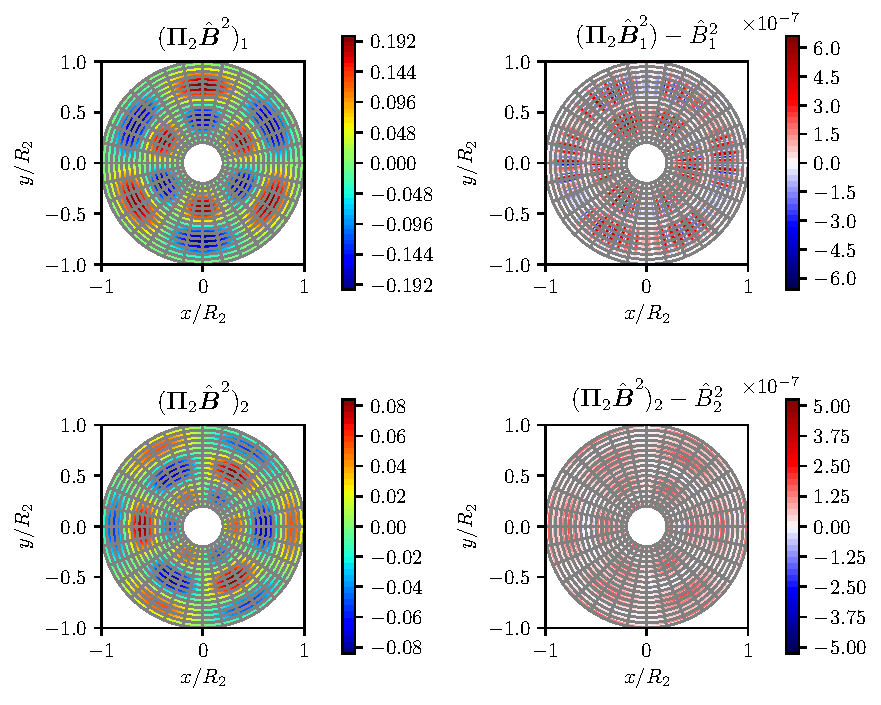
\includegraphics[scale=1.0]{projector_pi2.pdf}
\caption{Projection of the components (\ref{eq_components_projection_example}) using the projector (\ref{eq_proj2}) on an annulus defined by the mapping (\ref{eq_mapping_example}) obtained with B-splines of degree $p=(3,3,1)$. The number of elements $N_\text{el}=(128,256,2)$, number of quadrature points per integration interval $n_\text{q,pr}=(4,2,2)$ and number of quadrature points per element for the computation of (\ref{eq_L2error_V2}) $n_\text{q,el}=(4,2,2)$. Top: contour plots at $z=0.5L_z$ of the numerical 1-component (left) and error (right). Bottom: contour plots at $z=0.5L_z$ of the numerical 2-component (left) and error (right).\label{fig_projection_2form}}
\end{figure}
We choose the components
\begin{align}
\hat{\bo{B}}^2(\bo{\eta})=\begin{pmatrix}
\eta_1(1-\eta_1)\sin(2\pi\eta_1)\sin(6\pi\eta_2) \\
\frac{1}{6\pi}(1-2\eta_1)\sin(2\pi\eta_1) + \eta_1(1-\eta_1)\cos(2\pi\eta_1)2\pi]\cos(6\pi\eta_2)\\
0
\end{pmatrix},\label{eq_components_projection_example}
\end{align}
clamped B-splines for the radial-like coordinate $\eta_1$ and periodic B-splines for the angle-like coordinate $\eta_2$ as well as for $\eta_3$. We measure the error of the projected components compared to the exact ones in the $L^2$-norm of the space of 2-forms,
\begin{align}
||\Delta\hat{\bo{B}}^2||_{L^2}:=||\hat{\bo{B}}^2-\bo{\Pi}_2\hat{\bo{B}}^2||_{L^2}=\int_{\hat{\Omega}}(\hat{\bo{B}}^2-\bo{\Pi}_2\hat{\bo{B}}^2)^\top G (\hat{\bo{B}}^2-\bo{\Pi}_2\hat{\bo{B}}^2)\frac{1}{\sqrt{g}}\,\text{d}^3\eta,\label{eq_L2error_V2}
\end{align}
as we refine the mesh (that is, as we increase the number of elements), computed using Gauss-Legendre quadrature points. Furthermore, to verify the commuting diagram property, we estimate the spatial $L^\infty$-norm of $\hat{\nabla}\cdot \bo{\Pi}_2\hat{\bo{B}}^2$,
\begin{align}
||\hat{\nabla}\cdot\bo{\Pi}_2\hat{\bo{B}}^2||_{L^\infty}:=\underset{(\eta_1,\eta_2,\eta_3)\in\hat{\Omega}}{\text{max}}|\hat{\nabla}\cdot\bo{\Pi}_2\hat{\bo{B}}^2|,
\end{align}
at the Greville points \cite{Farin1993}. The resulting projected components are shown in Figure \ref{fig_projection_2form} for typical parameters. Table \ref{tab_convergence_pi2} shows the convergence of the projector while increasing the number of elements using quadratic and cubic splines. It can be seen that the divergence of the projected field is close to zero ($\approx10^{-13}$) for any spline degree and resolution. This shows that the commuting diagram property is satisfied exactly.
\begin{table}[H]
\renewcommand*{\arraystretch}{1.6}
\centering
\begin{tabular}{|c||ccc|ccc|}
\hline
&\multicolumn{3}{c|}{$p=(2,2,1)$} &\multicolumn{3}{c|}{$p=(3,3,1)$}\\
\hline
$N_\text{el}$ &$||\Delta\hat{\bo{B}}^2||_{L^2}$ &Order &$||\hat{\nabla}\cdot\bo{\Pi}_2\hat{\bo{B}}^2||_{L^\infty}$ &$||\Delta\hat{\bo{B}}^2||_{L^2}$ &Order &$||\hat{\nabla}\cdot\bo{\Pi}_2\hat{\bo{B}}^2||_{L^\infty}$  \\
\hline
$(32,64,2)$  &$2.75\cdot10^{-4}$ & &$4.23\cdot10^{-12}$ &$1.50\cdot10^{-5}$ & &$3.19\cdot10^{-14}$ \\
\hline
$(64,128,2)$ &$6.81\cdot10^{-5}$ &$2.01$ &$8.42\cdot10^{-14}$ &$1.56\cdot10^{-6}$ &$3.27$ &$6.02\cdot10^{-14}$ \\
\hline
$(128,256,2)$ &$1.70\cdot10^{-5}$ &$2.00$ &$4.97\cdot10^{-14}$ &$1.82\cdot10^{-7}$ &$3.10$ &$8.19\cdot10^{-14}$ \\
\hline
$(256,512,2)$ &$4.25\cdot10^{-6}$ &$2.00$ &$1.54\cdot10^{-13}$ &$2.21\cdot10^{-8}$ &$3.04$ &$2.76\cdot10^{-13}$\\
\hline
$(512,1024,2)$ &$1.06\cdot10^{-6}$ &$2.00$ &$3.42\cdot10^{-13}$ &$2.73\cdot10^{-9}$ &$3.02$ &$5.86\cdot10^{-13}$\\
\hline
\end{tabular}
\caption{Projection of the components (\ref{eq_components_projection_example}) using the projector (\ref{eq_proj2}) on an annulus defined by the mapping (\ref{eq_mapping_example}): $p$-th order convergence of the projector and divergence close to machine precision.\label{tab_convergence_pi2}}
\end{table}

\subsection{PIC coupling terms}
\label{sec_PIC}
We solve the Vlasov equation (\ref{eq_kinetics_linear}) with classical particle-in-cell techniques. Hence we assume a particle-like distribution function which, in physical space $\Omega$, takes the form
\begin{align}
f_\text{h}&=f_\text{h}(t,\bo{x},\bo{v})\approx\sum_{k=1}^{K}w_k\delta(\bo{x}-\bo{x}_k(t))\delta(\bo{v}-\bo{v}_k(t)),\label{eq_discrete_fh}
\end{align}
where $K$ is the total number of simulation markers (to which we simply refer to as particles), $w_k$ is the weight of the $k$-th particle and $\bo{x}_k=\bo{x}_k(t)$ and $\bo{v}_k=\bo{v}_k(t)$ its position in phase space at time $t$ satisfying the equations of motion
\begin{subequations}
\label{eq_PICmotion}
\begin{alignat}{2}
&\frac{\text{d}\bo{x}_k}{\text{d}t}=\bo{v}_k,&&\bo{x}_k(t=0)=\bo{x}_k^0,\\
&\frac{\text{d}\bo{v}_k}{\text{d}t}=\bo{B}(\bo{x}_k)\times\tilde{\bo{U}}(\bo{x}_k)+\bo{v}_k\times\bo{B}(\bo{x}_k),\qquad &&\bo{v}_k(t=0)=\bo{v}_k^0.
\end{alignat}
\end{subequations}

To transform the equations of motion (\ref{eq_PICmotion}) to logical spatial coordinates $\bo{\eta}_k$, we note that $\text{d}\bo{x}(\bo{\eta}(t))/\text{d}t=DF\text{d}\bo{\eta}/\text{d}t$ for the first equation. Regarding the second equation, we first write it in curvilinear coordinates ($\bo{B}=DF\hat{\bo{B}_\text{f}}$ and $\tilde{\bo{U}}=DF\hat{\bo{U}}$) and then use the relations (\ref{eq_transformation_diffforms}) to transform the components $\hat{\bo{B}}_\text{f}$ and $\hat{\bo{U}}$ the corresponding 2-form and 1-form components, respectively. Finally, we replace the continuous forms by their finite element approximations to obtain
\begin{subequations}
\label{eq_PICmotion_curv}
\begin{align}
\frac{\text{d}\bo{\eta}_k}{\text{d}t}&=DF^{-1}(\bo{\eta}_k)\bo{v}_k,\\
\frac{\text{d}\bo{v}_k}{\text{d}t}&=(DF^{-1}(\bo{\eta}_k))^\top\left[\hat{\bo{B}}_{\text{f}h}^2(\bo{\eta}_k)\times G^{-1}(\bo{\eta}_k)\hat{\bo{U}}_h^1(\bo{\eta}_k)-\hat{\bo{B}}_{\text{f}h}^2(\bo{\eta}_k)\times DF^{-1}(\bo{\eta}_k)\bo{v}_k\right].
\end{align} 
\end{subequations}
Here, we once more used the identity $M\bo{b}\times M\bo{c}=\text{det}(M) (M^{-1})^\top(\bo{b}\times\bo{c})$.

We now turn our attention to the two terms $\text{CC}(\rho_\text{h})$ and $\text{CC}(\bo{J}_\text{h})$ in the weak momentum balance equation (\ref{eq_momentum_weak}) involving the hot charge and current density. Following classical PIC techniques, the resulting integrals are evaluated by Monte-Carlo estimates using the particle positions in phase space \citep{Aydemir1993}. Explicitly,
\begin{align}
\text{CC}(\rho_\text{h})&\approx\int_{\hat{\Omega}}(\hat{\bo{C}}_h^1)^\top G^{-1}\hat{\rho}_\text{h}\left(\hat{\bo{B}}^2_{\text{f}h}\times G^{-1}\hat{\bo{U}}_h^1\right)\sqrt{g}\,\text{d}^3\eta\label{eq_PIC_term1}\\
&=\int_{\hat{\Omega}}\int_{\mathbb{R}^3}\left\lbrace(\hat{\bo{C}}_h^1)^\top G^{-1}\frac{\hat{f}_\text{h}}{\hat{s}_\text{h}}\left(\hat{\bo{B}}^2_{\text{f}h}\times G^{-1}\hat{\bo{U}}_h^1\right) \right\rbrace \hat{s}_\text{h}\sqrt{g}\,\text{d}^3 v\,\text{d}^3\eta\label{eq_PIC_randomvariable}\\
&\approx \sum_{k=1}^{K}\underbrace{\frac{1}{K}\frac{\hat{f}_\text{h}^0(\bo{\eta}^0_k,\bo{v}_k^0)}{\hat{s}_\text{h}^0(\bo{\eta}^0_k,\bo{v}_k^0)}}_{=:w_k}(\hat{\bo{C}}_h^1)^\top(\bo{\eta}_k)G^{-1}(\bo{\eta}_k)\left(\hat{\bo{B}}^2_{\text{f}h}(\bo{\eta}_k)\times G^{-1}(\bo{\eta}_k)\hat{\bo{U}}^1_{h}(\bo{\eta}_k)\right),\label{eq_PIC_estimator}
\end{align}
where we introduced the probability density function (PDF) $\hat{s}_\text{h}=\hat{s}_\text{h}(t,\bo{\eta},\bo{v})=s_\text{h}(t,\bo{F}(\bo{\eta}),\bo{v})$, which must be normalized to one and from which we demand to satisfy the Vlasov equation. Regarding the former, it is important to note that
\begin{align}
1=\int_{\Omega}\int_{\mathbb{R}^3}s_\text{h}(t,\bo{x},\bo{v})\,\text{d}^3x\,\text{d}^3v=\int_{\hat{\Omega}}\int_{\mathbb{R}^3}\hat{s}_\text{h}(t,\bo{\eta},\bo{v})\sqrt{g}(\bo{\bo{\eta}})\,\text{d}^3\eta\,\text{d}^3v,\qquad\quad\forall\,t\in\mathbb{R}^+_0,
\end{align}
such that the transformed PDF is given by $\tilde{s}_\text{h}:=\hat{s}_\text{h}\sqrt{g}$. Then (\ref{eq_PIC_randomvariable}) can be interpreted as the expectation value of the random variable inside the curly brackets distributed under the PDF $\tilde{s}_\text{h}$ with (\ref{eq_PIC_estimator}) being its estimator using the particle positions $(\bo{\eta}_k,\bo{v}_k)_{1\leq k\leq N_\text{p}}$ in phase space. Finally, we made use of the fact that $\hat{f}_\text{h}$ and $\hat{s}_\text{h}$ are constant along a particle trajectory according to the Vlasov equation, that is, $\text{d}\hat{f}_\text{h}/\text{d}t=0$ in a Lagrangian frame, i.e. $\hat{f}_\text{h}(t,\bo{\eta}_k(t),\bo{v}_k(t))=\hat{f}_\text{h}^0(\bo{\eta}^0_k,\bo{v}_k^0)$, where $\hat{f}_\text{h}^0=\hat{f}_\text{h}(t=0,\bo{\eta},\bo{v})=f_\text{h}(t=0,\bo{F}(\bo{\eta}),\bo{v})$ denotes the initial distribution function and $(\bo{\eta}_k^0,\bo{v}_k^0)$ is the initial position of the $k$-th particle in phase space drawn from the initial PDF $\hat{s}^0_\text{h}$. Hence the particle weights $(w_k)_{1\leq k\leq N_\text{p}}$ are constant in time which is not the case if, as shown in Appendix \ref{sec_appendix2}, a $\delta f$ approach is used. One should keep in mind that if one samples from the transformed PDF $\tilde{s}_\text{h}$, one must not forget the Jacobian determinant in the definition of the weights.

In order to write ($\ref{eq_PIC_estimator}$) as well as (\ref{eq_PICmotion_curv}) in matrix-vector form, we introduce the following vectors and matrices:
\begin{itemize}
\item {\makebox[1.7cm][l]{$\bo{H}$} \makebox[11cm][l]{$:=(\eta_{1,1},\cdots,\,\eta_{K,1},\eta_{1,2},\cdots,\,\eta_{K,2},\,\eta_{1,3},\cdots,\,\eta_{K,3})^\top$} $\in\mathbb{R}^{3K}$,}
\item {\makebox[1.7cm][l]{$\bo{V}$} \makebox[11cm][l]{$:=(v_{1,x},\cdots,\,v_{K,x},v_{1,y},\cdots,\,v_{K,y},\,v_{1,z},\cdots,\,v_{K,z})^\top$} $\in\mathbb{R}^{3K}$,}
\item {\makebox[1.7cm][l]{$\mathbb{W}$} \makebox[11cm][l]{$:=\mathbb{I}_3\otimes\text{diag}(w_1,\cdots,w_{K})$} $\in\mathbb{R}^{3K\times 3K}$,}
\item {\makebox[1.7cm][l]{$\mathbb{P}^n_\mu(\bo{H})$} \makebox[11cm][l]{$:=(\Lambda^n_{\mu,i}(\bo{\eta}_k))_{0\leq i\leq N_{\mu}^n-1,1\leq k\leq K}$ \hspace{1cm} ($n\in\{1,2\}$, $\mu\in\{1,2,3\})$} $\in\mathbb{R}^{N^n_{\mu}\times K}$,}
\item {\makebox[1.7cm][l]{$\mathbb{P}^n(\bo{H})$} \makebox[11cm][l]{$:=\text{diag}(\mathbb{P}^n_1,\,\mathbb{P}^n_2,\,\mathbb{P}^n_3)$\hspace{3.02cm} ($n\in\{1,2\}$)} $\in\mathbb{R}^{N^n\times 3K}$,}
\item {\makebox[1.7cm][l]{$\bar{G}^{-1}_{ab}(\bo{H})$} \makebox[11cm][l]{$:=\text{diag}(G^{-1}_{ab}(\bo{\eta}_1),\cdots,G^{-1}_{ab}(\bo{\eta}_{K}))$\hspace{0.85cm} ($a,b\in\{1,2,3\}$)} $\in\mathbb{R}^{K\times K}$,}
\item {\makebox[1.7cm][l]{$\bar{G}^{-1}(\bo{H})$} \makebox[11cm][l]{$:=(\bar{G}^{-1}_{ab})_{1\leq a,b\leq 3}$} $\in\mathbb{R}^{3K\times 3K}$,}
\item {\makebox[1.7cm][l]{$\bar{DF}^{-1}_{ab}(\bo{H})$} \makebox[11cm][l]{$:=\text{diag}(DF^{-1}_{ab}(\bo{\eta}_1),\cdots,DF^{-1}_{ab}(\bo{\eta}_{K}))$\quad ($a,b\in\{1,2,3\}$)} $\in\mathbb{R}^{K\times K}$,}
\item {\makebox[1.7cm][l]{$\bar{DF}^{-1}(\bo{H})$} \makebox[11cm][l]{$:=(\bar{DF}^{-1}_{ab})_{1\leq a,b\leq 3}$} $\in\mathbb{R}^{3K\times 3K}$,}
\item {\makebox[1.7cm][l]{$\mathbb{B}_{\text{f},\mu}(\mb{b},\bo{H})$} \makebox[11cm][l]{$:=\text{diag}(\mb{b}_\mu^\top\mathbb{P}^2_\mu)+\text{diag}(\hat{B}_{\text{eq},\mu}(\bo{\eta}_1),\cdots,\hat{B}_{\text{eq},\mu}(\bo{\eta}_{K}))$\quad$\mu\in\{1,2,3\}$} $\in\mathbb{R}^{K\times K}$,}
\end{itemize}
where $\mathbb{I}_3\in\mathbb{R}^{3\times 3}$ denotes the three-dimensional identity matrix and $\otimes$ the Kronecker product. In accordance with (\ref{eq_matrix_cross}), we additionally define the block matrix
\begin{align}
\mathbb{B}_\text{f}=\mathbb{B}_\text{f}(\mb{b},\bo{H}):=\begin{pmatrix}
0 &-\mathbb{B}_{\text{f},3} &\phantom{-}\mathbb{B}_{\text{f},2} \\
\phantom{-}\mathbb{B}_{\text{f},3} &0 &-\mathbb{B}_{\text{f},1} \\
-\mathbb{B}_{\text{f},2} &\phantom{-}\mathbb{B}_{\text{f},1} &0
\end{pmatrix}\in\mathbb{R}^{3K\times 3NK},
\end{align} 
which represents the cross product with the total magnetic field at all particle positions. With this (\ref{eq_PIC_estimator}) becomes
\begin{align}
\text{CC}(\rho_\text{ch})\approx \mb{c}^\top\mathbb{P}^1\mathbb{W}\bar{G}^{-1}\mathbb{B}_\text{f}\bar{G}^{-1}(\mathbb{P}^1)^\top\mb{u}.
\end{align}
The same procedure holds for the term involving the hot current density:
\begin{align}
\text{CC}(\bo{J}_\text{h})&\approx\int_{\hat{\Omega}}(\hat{\bo{C}}_h^1)^\top G^{-1}\left(\hat{\bo{B}}_{\text{f}h}^2\times\hat{\bo{J}}_\text{h}\right)\sqrt{g}\,\text{d}^3\eta\\
&=\int_{\hat{\Omega}}\int_{\mathbb{R}^3}\left\lbrace(\hat{\bo{C}}_h^1)^\top G^{-1}\frac{\hat{f}_\text{h}}{\hat{s}_\text{h}}\left(\hat{\bo{B}}_{\text{f}h}^2\times DF^{-1}\bo{v}\right)\right\rbrace\hat{s}_\text{h}\sqrt{g}\,\text{d}^3v\,\text{d}^3\eta\\
&\approx \sum_{k=1}^{N_\text{p}}w_k(\hat{\bo{C}}_h^1)^\top(\bo{\eta}_k)G^{-1}(\bo{\eta}_k)\left(\hat{\bo{B}}^2_{\text{f}h}(\bo{\eta}_k)\times DF^{-1}(\bo{\eta}_k)\bo{v}_k\right)\\
&=\mb{c}^\top\mathbb{P}^1\mathbb{W}\bar{G}^{-1}\mathbb{B}_{\text{f}}\bar{DF}^{-1}\bo{V}.
\end{align}
Collecting the terms (\ref{eq_matrix_momentum1}), (\ref{eq_matrix_momentum2}), (\ref{eq_curl_background}) and (\ref{eq_matrix_momentum4}), we find in summary the following semi-discrete momentum balance equation:
\begin{align}
\mathcal{A}\dot{\mb{u}}=\mathcal{T}^\top\mathbb{C}^\top\mathbb{M}^2\mb{b}+\mathbb{M}^1\mathcal{P}\mb{b}-\mathbb{P}^1\mathbb{W}\bar{G}^{-1}\mathbb{B}_\text{f}\bar{G}^{-1}(\mathbb{P}^1)^\top\mb{u}+\mathbb{P}^1\mathbb{W}\bar{G}^{-1}\mathbb{B}_{\text{f}}\bar{DF}^{-1}\bo{V}-\mathbb{M}^1\mathbb{G}\mb{p}.\label{eq_momentum_semi}
\end{align}
Finally, we also write the equations of motion (\ref{eq_PICmotion_curv}) of all particles in a compact matrix-vector form:
\begin{subequations}
\label{eq_PICmotion_matrix}
\begin{align}
&\frac{\text{d}\bo{H}}{\text{d}t}=\bar{DF}^{-1}(\bo{H})\bo{V},\\
&\frac{\text{d}\bo{V}}{\text{d}t}=(\bar{DF}^{-1}(\bo{H}))^\top\left[\mathbb{B}_\text{f}(\mb{b},\bo{H})\bar{G}^{-1}(\bo{H})(\mathbb{P}^1)^\top(\bo{H})\mb{u}-\mathbb{B}_\text{f}(\mb{b},\bo{H})\bar{DF}^{-1}(\bo{H})\bo{V}\right].
\end{align}
\end{subequations}


\subsection{Energy and Hamiltonian system}
Let us define the discrete energy corresponding to (\ref{eq_Hamiltonian1_linear}). We use the same splitting (\ref{eq_split_inertia}) for the kinetic energy of the bulk plasma in order to end up with the same matrix $\mathcal{A}$ as in the semi-discrete momentum balance equation (\ref{eq_momentum_semi}):
\begin{align}
\begin{split}
\mathcal{H}_{1h}:&=\frac{1}{4}\intom\left[\bo{\Pi}_1\left(\frac{\hat{\rho}_\text{eq}^3}{\sqrt{g}}\hat{\bo{U}}_h^1\right)\right]^\top\hspace{-2mm} G^{-1}\hat{\bo{U}}_h^1\sqrt{g}\,\text{d}^3\eta+\frac{1}{4}\intom\left(\hat{\bo{U}}_h^1\right)^\top\hspace{-2mm}G^{-1}\bo{\Pi}_1\left(\frac{\hat{\rho}_\text{eq}^3}{\sqrt{g}}\hat{\bo{U}}_h^1\right)\sqrt{g}\,\text{d}^3\eta\\
&\hspace{1.5cm}+\frac{1}{2}\int_{\hat{\Omega}}(\hat{\bo{B}}_h^2)^\top G\hat{\bo{B}}_h^2\frac{1}{\sqrt{g}}\,\text{d}^3\eta+\frac{1}{\gamma-1}\int_{\hat{\Omega}}\hat{p}^0_h\sqrt{g}\,\text{d}^3\eta+\frac{1}{2}\int_{\hat{\Omega}}\int_{\mathbb{R}^3} v^2f_\text{h}\,\text{d}^3v\,\text{d}^3x\\
&=\frac{1}{2}\mb{u}^\top\mathcal{A}\mb{u}+\frac{1}{2}\mb{b}^\top\mathbb{M}^2\mb{b}+\frac{1}{\gamma-1}\mb{p}^\top\mb{n}+\frac{1}{2}\bo{V}^\top\mathbb{W}\bo{V}.
\end{split}
\end{align}
The expression for the energy of the kinetic species (last term) is simply obtained by using the discrete distribution function (\ref{eq_discrete_fh}) and evaluating the integrals. The vector $\mb{n}$ contains all integrals of each basis function in $V_0$ over $\hat{\Omega}$, i.e.
\begin{align}
\mb{n}:=\left(\int_{\hat{\Omega}}\Lambda^0_0\sqrt{g}\,\text{d}^3\eta,\cdots,\int_{\hat{\Omega}}\Lambda^0_{N^0-1}\sqrt{g}\,\text{d}^3\eta\right)^\top.
\end{align}
If we collect all finite element coefficients and particle positions in phase space in a single vector $\mb{R}^\top:=(\bo{\rho}^\top,\mb{u}^\top,\mb{p}^\top,\mb{b}^\top,\bo{H}^\top,\bo{V}^\top)\in\mathbb{R}^{N^3+N^1+N^0+N^2+3N_\text{p}+3N_\text{p}}$, we can write the semi-discrete MHD equations (\ref{eq_continuity_semi}), (\ref{eq_induction_discrete2}), (\ref{eq_pressure_semi}) and (\ref{eq_momentum_semi}) and PIC equations (\ref{eq_PICmotion_matrix}) in the following compact form:
\begin{align}
\begin{split}
&\frac{\text{d}\mb{R}}{\text{d}t}=\mathbb{J}\nabla_\mb{R}\mathcal{H}_{1h}+\mathbb{K}\mb{R}=
\begin{pmatrix}
0 &0 &0 &0 &0 &0 \\
0 &\textcolor{red}{\mathbb{J}_{11}(\mb{b},\boldsymbol{H})} &\textcolor{blue}{\mathbb{J}_{12}} &0 &0 &\textcolor{green}{\mathbb{J}_{14}(\mb{b},\boldsymbol{H})}\\
0 &0 &0 &0 &0 &0 \\
0 &\textcolor{blue}{-\mathbb{J}_{12}^\top} &0 &0 &0 &0 \\
0 &0 &0 &0 &0 &\textcolor{magenta}{\mathbb{J}_{34}(\boldsymbol{H})} \\
0 &\textcolor{green}{-\mathbb{J}_{14}^\top(\mb{b},\boldsymbol{H})} &0 &0 &\textcolor{magenta}{-\mathbb{J}_{34}^\top(\boldsymbol{H})} &\mathbb{J}_{44}(\mb{b},\boldsymbol{H})
\end{pmatrix}\begin{pmatrix}
0\\
\mathcal{A}\mb{u} \\
0 \\
\mathbb{M}^2\mb{b}\\
0 \\
\mathbb{W}\mb{V}
\end{pmatrix}\\[2mm]
&\hspace{1.5cm}+\begin{pmatrix}
0 &-\mathbb{D}\mathcal{Q} &0 &0 &0 &0 \\
0 &0 &\mathcal{A}^{-1}\mathbb{M}^1\mathcal{P} &-\mathcal{A}^{-1}\mathbb{M}^1\mathbb{G} &0 &0 \\
0 &(\mathbb{M}^0)^{-1}\left[\mathbb{G}^\top\mathbb{M}^1\mathcal{S}+(\gamma-1)\mathcal{K}^\top\mathbb{G}^\top\mathbb{M}^1\right] &0 &0 &0 &0 \\
0 &0 &0 &0 &0 &0 \\
0 &0 &0 &0 &0 &0 \\
0 &0 &0 &0 &0 &0
\end{pmatrix}\begin{pmatrix}
\boldsymbol{\rho}\\
\mb{u} \\
\mb{p} \\
\mb{b}\\
\boldsymbol{H} \\
\mb{V}
\end{pmatrix}.
\end{split}
\end{align}
We find that our spatial discretization results in a system which can be written as the sum of a non-canonical Hamiltonian part with the Poisson matrix $\mathbb{J}$ and a non-Hamiltonian part with the matrix $\mathbb{K}$. As already mentioned in Section \ref{sec_model}, the latter only plays a role for compressible waves and if $\nabla\times\bo{B}_\text{eq}\neq 0$ (then $\mathcal{P}=0$). In particular, we remark that obtaining the Hamiltonian part relies on the symmetry of $\mathcal{A}$, $\mathbb{M}^2$ and $\mathbb{W}$. While it obvious for the last two matrices, the symmetry of $\mathcal{A}$ is ensured by the splitting performed in (\ref{eq_split_inertia}). In in this case the anti-symmetry of $\mathbb{J}$ immediately implies conservation of $\mathcal{H}_{1h}$. The single blocks of $\mathbb{J}$ are given by
\begin{subequations}
\begin{align}
\textcolor{red}{\mathbb{J}_{11}(\mb{b},\bo{H})}&=-\mathcal{A}^{-1}\mathbb{P}^1(\bo{H})\mathbb{W}\bar{G}^{-1}(\bo{\boldsymbol{H}})\mathbb{B}_\text{f}(\mb{b},\bo{H})\bar{G}^{-1}(\bo{H})(\mathbb{P}^1)^\top(\bo{H})\mathcal{A}^{-1},\\[1mm]
\textcolor{blue}{\mathbb{J}_{12}}&=\mathcal{A}^{-1}\mathcal{T}^\top\mathbb{C}^\top,\\[1mm]
\textcolor{green}{\mathbb{J}_{14}(\mb{b},\bo{H})}&=\mathcal{A}^{-1}\mathbb{P}^1(\bo{H})\tilde{G}^{-1}(\bo{H})\mathbb{B}_\text{f}(\mb{b},\bo{H})\tilde{DF}^{-1}(\bo{H}),\\
\textcolor{magenta}{\mathbb{J}_{34}(\bo{H})}&=\bar{DF}^{-1}(\bo{H})\mathbb{W}^{-1},\\
\mathbb{J}_{44}(\mb{b},\bo{H})&=-(\tilde{DF}^{-1})^\top(\bo{H})\mathbb{B}_\text{f}(\mb{b},\bo{H})\tilde{DF}^{-1}(\bo{H})\mathbb{W}^{-1}.
\end{align}
\end{subequations}


\section{Time discretization}
\label{sec_time}
In order to keep the energy conservation property, we propose two splitting steps: First, we split apart the non-Hamiltonian part $\mathbb{K}\mb{R}$, and second, we apply Poisson splitting to the Hamiltonian part $\mathbb{J}\nabla_\mb{R}\mathcal{H}_{1\text{h}}$ and solve each (anti-symmetric) sub-step in an energy conserving way. We recall the Hamiltonian part:
\begin{align}
&\frac{\text{d}}{\text{d}t}\begin{pmatrix}
\mb{u} \\ \mb{b} \\ \bo{H} \\ \bo{V}
\end{pmatrix}=
\begin{pmatrix}
\textcolor{red}{\mathbb{J}_{11}(\mb{b},\bo{H})} &\textcolor{blue}{\mathbb{J}_{12}} &0 &\textcolor{green}{\mathbb{J}_{14}(\mb{b},\bo{H})}\\
\textcolor{blue}{-\mathbb{J}_{12}^\top} &0 &0 &0 \\
0 &0 &0 &\textcolor{magenta}{\mathbb{J}_{34}(\bo{H})} \\
\textcolor{green}{-\mathbb{J}_{14}^\top(\mb{b},\bo{H})} &0 &\textcolor{magenta}{-\mathbb{J}_{34}^\top(\bo{H})} &\mathbb{J}_{44}(\mb{b},\bo{H})
\end{pmatrix}\begin{pmatrix}
\mathcal{A}\mb{u} \\
\mathbb{M}^2\mb{b}\\
0 \\
\mathbb{W}\bo{V}
\end{pmatrix}.\label{eq_Poissonmatrix}
\end{align}
Introducing a temporal grid $t_n=n\Delta t$ with $n\in\mathbb{N}_0$ yields to following sub-steps:
\paragraph{Sub-step 1}
The first sub-system reads
\begin{align}
\dot{\mb{u}}=\mathbb{J}_{11}(\mb{b},\bo{H})\mathcal{A}\mb{u},\qquad\dot{\mb{b}}=0,\qquad\dot{\bo{H}}=0,\qquad\dot{\bo{V}}=0.\label{eq_timestep1}
\end{align}
We solve the equation for $\mb{u}$ with the energy-preserving, implicit Crank-Nicolson method \cite{Cranketal1947}. $\mathbb{J}_{11}=\mathbb{J}_{11}(\mb{b}^n,\bo{H}^n)$ remains constant in this step:
\begin{align}
\mb{u}^{n+1}&=\mb{u}^n+\frac{\Delta t}{2}\mathbb{J}_{11}(\mb{b}^n,\bo{H}^n)\mathcal{A}(\mb{u}^n+\mb{u}^{n+1}),\\
\Leftrightarrow \quad \left(\mathbb{I}-\frac{\Delta t}{2}\mathbb{J}_{11}(\mb{b}^n,\bo{H}^n)\mathcal{A}\right)\mb{u}^{n+1}&=\left(\mathbb{I}+\frac{\Delta t}{2}\mathbb{J}_{11}(\mb{b}^n,\bo{H}^n)\mathcal{A}\right)\mb{u}^n.
\end{align}
To avoid multiple matrix inversions, we multiply the second line with $\mathcal{A}$ from the left-hand side to obtain 
\begin{align}
\left(\mathcal{A}-\frac{\Delta t}{2}\mathcal{A}\mathbb{J}_{11}(\mb{b}^n,\bo{H}^n)\mathcal{A}\right)\mb{u}^{n+1}=\left(\mathcal{A}+\frac{\Delta t}{2}\mathcal{A}\mathbb{J}_{11}(\mb{b}^n,\bo{H}^n)\mathcal{A}\right)\mb{u}^n.
\end{align}
We denote the corresponding integrator by $\Phi_{\Delta t}^1:\mathbb{R}^{N^1}\rightarrow\mathbb{R}^{N^1},\,\mb{u}^n\mapsto\mb{u}^{n+1}$.
\paragraph{Sub-step 2}
The second sub-system reads
\begin{align}
\dot{\mb{u}}=\mathbb{J}_{12}\mathbb{M}^2\mb{b},\qquad\dot{\mb{b}}=-\mathbb{J}_{12}^\top\mathcal{A}\mb{u},\qquad\dot{\bo{H}}=0,\qquad\dot{\bo{V}}=0.
\end{align}
As before, we solve this system with the Crank-Nicolson method,\label{eq_timestep2}
\begin{align}
&\mb{u}^{n+1}=\mb{u}^n+\frac{\Delta t}{2}\mathcal{A}^{-1}\mathcal{T}^\top\mathbb{C}^\top(\mb{b}^n+\mb{b}^{n+1}),\\
&\mb{b}^{n+1}=\mb{b}^n-\frac{\Delta t}{2}\mathbb{C}\mathcal{T}\Delta t(\mb{u}^n+\mb{u}^{n+1}),
\end{align}
ans solve for $\mb{u}^{n+1}$ by plugging the second into the first equation. After some straightforward manipulations this results in
\begin{align}
&\mb{u}^{n+1}=S_2^{-1}\left[\left(\mathcal{A}-\frac{\Delta t^2}{4}\mathcal{T}^\top\mathbb{C}^\top\mathbb{M}^2\mathbb{C}\mathcal{T}\right)\mb{u}^{n}+\Delta t\mathcal{T}^\top\mathbb{C}^\top\mathbb{M}^2\mb{b}^n\right],\\
&\mb{b}^{n+1}=\mb{b}^n-\frac{\Delta t}{2}\mathbb{C}\mathcal{T}(\mb{u}^n+\mb{u}^{n+1}),\label{eq_updateb}
\end{align}
where $S_2:=\mathcal{A}+\Delta t^2\mathcal{T}^\top\mathbb{C}^\top\mathbb{M}^2\mathbb{C}\mathcal{T}/4$. Particularly, we note the explicit update rule for $\mb{b}$ which preserves the divergence-free constraint, i.e. $\mathbb{D}\mb{b}^{n+1}=\mathbb{D}\mb{b}^{n}$ due to $\mathbb{D}\mathbb{C}=0$. We denote the corresponding integrator by $\Phi_{\Delta t}^2:\mathbb{R}^{N^1}\times\mathbb{R}^{N^2}\rightarrow\mathbb{R}^{N^1}\times\mathbb{R}^{N^2},\,\mb{u}^n,\mb{b}^n\mapsto\mb{u}^{n+1},\mb{b}^{n+1}$.
\paragraph{Sub-step 3}
The third sub-system reads
\begin{align}
\dot{\mb{u}}=\mathbb{J}_{14}(\mb{b},\bo{H})\mathbb{W}\bo{V},\qquad\dot{\mb{b}}=0,\qquad\dot{\bo{H}}=0,\qquad\dot{\bo{V}}=-\mathbb{J}_{14}^\top(\mb{b},\bo{H})\mathcal{A}\mb{u}.\label{eq_timestep3}
\end{align}
We solve this system in the same way as before. Since $\mb{b}$ and $\bo{H}$ do not change in this step, the same is true for the matrix $\mathbb{J}_{14}$. Hence $\mathbb{J}_{14}=\mathbb{J}_{14}(\mb{b}^n,\bo{H}^n)$ and we have
\begin{align}
\mb{u}^{n+1}&=\mb{u}^n+\frac{\Delta t}{2}\mathbb{J}_{14}\mathbb{W}(\bo{V}^n+\bo{V}^{n+1}),\\
\bo{V}^{n+1}&=\bo{V}^n-\frac{\Delta t}{2}\mathbb{J}_{14}^\top(\mb{u}^n+\mb{u}^{n+1}),\\[5mm]
\Leftrightarrow\quad\mb{u}^{n+1}&=S^{-1}_3\left[\left(\mathcal{A}-\frac{\Delta t^2}{4}\mathcal{A}\mathbb{J}_{14}\mathbb{W}\mathbb{J}_{14}^\top\mathcal{A}\right)\mb{u}^{n}+\Delta t\mathcal{A}\mathbb{J}_{14}\mathbb{W}\bo{V}^n\right],\\
\Leftrightarrow\quad\bo{V}^{n+1}&=\bo{V}^n-\frac{\Delta t}{2}\mathbb{J}_{14}^\top\mathcal{A}(\mb{u}^n+\mb{u}^{n+1}),
\end{align}
where $S_3:=\mathcal{A}+\Delta t^2\mathcal{A}\mathbb{J}_{14}\mathbb{W}\mathbb{J}_{14}^\top\mathcal{A}/4$. We denote the corresponding integrator by $\Phi_{\Delta t}^3:\mathbb{R}^{N^1}\times\mathbb{R}^{3N_\text{p}}\rightarrow\mathbb{R}^{N^1}\times\mathbb{R}^{3N_\text{p}},\,\mb{u}^n,\bo{V}^n\mapsto\mb{u}^{n+1},\bo{V}^{n+1}$.
\paragraph{Sub-step 4}
The fourth sub-system reads
\begin{align}
\dot{\mb{u}}=0,\qquad\dot{\mb{b}}=0,\qquad\dot{\bo{H}}=\bar{DF}^{-1}(\bo{H})\bo{V},\qquad\dot{\bo{V}}=0.\label{eq_timestep4}
\end{align}
Since this step does not play a role for conservation of energy (the discrete Hamiltonian does not depend on the particle spatial coordinates), we apply to this system a standard fourth order Runge-Kutta scheme and denote the integrator by $\Phi_{\Delta t}^4:\mathbb{R}^{3N_\text{p}}\times\mathbb{R}^{3N_\text{p}},\,\bo{H}^n\mapsto\bo{H}^{n+1}$.
\paragraph{Sub-step 5}
The fifth sub-system reads
\begin{align}
\dot{\mb{u}}=0,\qquad\dot{\mb{b}}&=0,\qquad\dot{\bo{H}}=0,\qquad\dot{\bo{V}}=\mathbb{J}_{44}(\mb{b},\bo{H})\mathbb{W}\mb{V}.\label{eq_timestep5}
\end{align}
Using once more the Crank-Nicolson scheme yields
\begin{align}
\begin{split}
&\left[\mathbb{I}+\frac{\Delta t}{2}(\bar{DF}^{-1}(\bo{H}^n))^\top\mathbb{B}_\text{f}(\mb{b}^n,\bo{H}^n)\bar{DF}^{-1}(\bo{H}^n)\right]\bo{V}^{n+1}\\
&\hspace{4cm}=\left[\mathbb{I}-\frac{\Delta t}{2}(\bar{DF}^{-1}(\bo{H}^n))^\top\mathbb{B}_\text{f}(\mb{b}^n,\bo{H}^n)\bar{DF}^{-1}(\bo{H}^n)\right]\bo{V}^{n}
\end{split}
\end{align}
We denote the corresponding integrator by $\Phi_{\Delta t}^5:\mathbb{R}^{3N_\text{p}}\times\mathbb{R}^{3N_\text{p}},\,\bo{V}^{n}\mapsto\bo{V}^{n+1}$.
\paragraph{Sub-step 6 (Non-Hamiltonian part)}
The sixth sub-system reads
\begin{align}
\dot{\bo{\rho}}=-\mathbb{D}\mathcal{Q}\mb{u},\hspace{-1mm}\qquad\mathcal{A}\dot{\mb{u}}&=-\mathbb{M}^1\mathbb{G}\mb{p}+\mathbb{M}^1\mathcal{P}\mb{b},\hspace{-1mm}\qquad\mathbb{M}^0\dot{\mb{p}}=\left[\mathbb{G}^\top\mathbb{M}^1\mathcal{S}+(\gamma - 1)\mathcal{K}^\top\mathbb{G}^\top\mathbb{M}^1\right]\mb{u},\hspace{-1mm}\qquad\dot{\mb{b}}=0.\label{eq_timestep6}
\end{align}
Defining $\mathbb{L}:=\mathbb{G}^\top\mathbb{M}^1\mathcal{S}+(\gamma - 1)\mathcal{K}^\top\mathbb{G}^\top\mathbb{M}^1$ for a shorter notation, we solve this again with the Crank-Nicolson method:
\begin{align}
\bo{\rho}^{n+1}&=\bo{\rho}^n-\frac{\Delta t}{2}\mathbb{D}\mathcal{Q}(\mb{u}^{n+1}+\mb{u}^n),\label{eq_timestep6_rho}\\
\begin{pmatrix}
\mathcal{A} &\frac{\Delta t}{2}\mathbb{M}^1\mathbb{G}\\
-\frac{\Delta t}{2}\mathbb{L} &\mathbb{M}^0
\end{pmatrix}\begin{pmatrix}
\mb{u}^{n+1}\\ \mb{p}^{n+1}
\end{pmatrix}&=\begin{pmatrix}
\mathcal{A} &-\frac{\Delta t}{2}\mathbb{M}^1\mathbb{G}\\
\frac{\Delta t}{2}\mathbb{L} &\mathbb{M}^0
\end{pmatrix}\begin{pmatrix}
\mb{u}^{n}\\ \mb{p}^{n}
\end{pmatrix}+\begin{pmatrix}
\Delta t\mathbb{M}^1\mathcal{P}\mb{b}^n\\0
\end{pmatrix}.\label{eq_timestep6_up}
\end{align}
Hence, we first compute $\mb{u}^{n+1}$ and $\mb{p}^{n+1}$ from (\ref{eq_timestep6_up}) and then $\bo{\rho}^{n+1}$ from (\ref{eq_timestep6_rho}). Note that (\ref{eq_timestep6_rho}) implies exact conservation of mass due to the same argument as in (\ref{eq_mass_coservation_semi}), namely that the basis functions in $V_3$ are all normalized to one on the logical domain $\hat{\Omega}$. Consequently, the discrete mass is just the sum of the coefficients $\bo{\rho}$ and from (\ref{eq_timestep6_rho}) it follows that
\begin{align}
\sum_{i=0}^{N^3-1}\rho_i^{n+1}=\sum_{i=0}^{N^3-1}\rho_i^{n},
\end{align}
due to the form of $\mathbb{D}$ containing only $1$, $-1$ and $0$. We denote the corresponding integrator by $\Phi_{\Delta t}^6:\mathbb{R}^{N^3}\times\mathbb{R}^{N^1}\times\mathbb{R}^{N^0}\rightarrow\mathbb{R}^{N^3}\times\mathbb{R}^{N^1}\times\mathbb{R}^{N^0},\,\bo{\rho}^n,\mb{u}^n,\mb{p}^n\mapsto\bo{\rho}^{n+1},\mb{u}^{n+1},\mb{p}^{n+1}$. 

In summary, in order to go from time step $t_n$ to $t_{n+1}$, we successively apply the six integrators, where it is important to note that the input of the next integrator must be the output of the previous integrator:
\begin{align}
\Phi_{\Delta t}:=\Phi_{\Delta t}^6\circ\Phi_{\Delta t}^5\circ\Phi_{\Delta t}^4\circ\Phi_{\Delta t}^3\circ\Phi_{\Delta t}^2\circ\Phi_{\Delta t}^1.
\end{align}
This first-order compositions is also know as the Lie-Trotter splitting \cite{}. We remark, however, that higher-order compositions are available and can be found e.g. in \cite{McLachlanetal2012}.´

\section{Numerical experiments}
\label{sec_experiments}
\begin{figure}
\centering
\includegraphics[scale=1.0]{Cartesian_mesh.pdf}\hspace{1.5cm}
\includegraphics[scale=1.0]{Colella_mesh.pdf}
\caption{Exemplary meshes in the $xy-$ plane corresponding to the two mappings defined in (\ref{eq_mappings_exp}). For the Colella mapping (right) the parameter $\alpha=0.06$.\label{fig_meshes}}
\end{figure}
In this section we present a collection of numerical results obtained with the techniques shown in the previous sections. Here, we shall use only two types of mappings, where the first one is a standard Cartesian mapping $\bo{F}_\text{Ca}$ which we we use as a reference and the second one a so-called Colella mapping $\bo{F}_\text{Co}$ with which we test the impact of a distortion of the finite element mesh:
\begin{align}
\bo{F}_\text{Ca}:\hat{\Omega}\rightarrow\Omega,\bo{\eta}\mapsto\begin{pmatrix}
L_x\eta_1\\
L_y\eta_2\\
L_z\eta_3
\end{pmatrix}=\bo{x},\quad\bo{F}_\text{Co}:\hat{\Omega}\rightarrow\Omega,\bo{\eta}\mapsto\begin{pmatrix}
L_x(\eta_1+\alpha\sin(2\pi\eta_1)\sin(2\pi\eta_2))\\
L_y(\eta_2+\alpha\sin(2\pi\eta_2)\sin(2\pi\eta_3))\\
L_z\eta_3
\end{pmatrix}=\bo{x}.\label{eq_mappings_exp}
\end{align}
Here, $L_x,L_y,L_z>0$ are the side lengths of the rectangular physical domain $\Omega$ and $0\leq\alpha<1/(2\pi)$ is a parameter describing the distortion of the mesh. The upper limit for $\alpha$ is chosen such that the mapping does not become singular anywhere in the domain $\Omega$. Note that all quantities related to the mapping, such as the Jacobian determinant or the metric tensor, are constant and diagonal in case of the Cartesian mapping. Both is not true anymore in case of the Colella mapping. Figure \ref{fig_meshes} displays the resulting coordinate lines in the $xy$-plane and we note that the Colella mapping collapses to the Cartesian mapping for $\alpha=0$.

Furthermore, in all simulations shown, we assume a uniform equilibrium bulk plasma in physical space\footnote{Note that in case of the Colella mapping this is not true for the components of the corresponding differential forms on the logical domain.}. The first two subsections focus on linear MHD waves and linear wave-particle interactions. In contrast to that, the third subsection focuses on longer simulations deep into the nonlinear phase.
\subsection{Pure MHD}
In this paragraph we set the contribution from the kinetic ions to zero ($f_\text{h}=0$ for all times) and investigate linear MHD waves within the framework of STRUPHY. The dispersion relation for waves propagating in the $x$-direction ($\bo{k}=k\bo{e}_x$) in a homogeneous plasma of pressure $p_\text{eq}$ and density $\rho_\text{eq}$ in a magnetic field $\bo{B}_\text{eq}=B_{0x}\bo{e}_x+B_{0y}\bo{e}_y$ reads
\begin{align}
\left(\omega^2-k^2v_\text{A}^2\frac{B_{0x}^2}{B_{0x}^2+B_{0y}^2}\right)\left[\omega^2-\frac{1}{2}k^2(c_\text{S}^2+v_\text{A}^2)(1\pm\sqrt{1 - \delta})\right]=0,\quad\delta=\frac{4B_{0x}^2c_\text{S}^2v_\text{A}^2}{(c_\text{S}^2+v_\text{A}^2)^2(B_{0x}^2+B_{0y}^2)},
\end{align}
where the first term in the rounds brackets represents the shear Alfvén wave and the second term in the square brackets the slow (-) and fast (+) magnetosonic wave, respectively. The two characteristic velocities are the Alfvén velocity $v_\text{A}^2=(B_{0x}^2+B_{0y}^2)/(\mu_0\rho_\text{eq})$ and the speed of sound $c_\text{S}^2=\gamma p_\text{eq}/\rho_\text{eq}$.
\begin{figure}
\centering
\includegraphics[scale=1.0]{pure_MHD_timestep.pdf}
\caption{Normalized MHD power spectra in the $\omega-k_x$-plane for different time steps obtained by initialization with white noise. Parameters are $N_\text{el}=(80,80,2)$, $p=(3,3,1)$, $L_x=L_y=2000 \,v_\text{A}/\Omega_\text{ci}$, $L_z=5 \,v_\text{A}/\Omega_\text{ci}$, periodic boundary conditions everywhere, $n_\text{q,el}=(6,6,2)$ and $n_\text{pr,el}=(6,6,2)$. Dashed black lines are the analytical dispersion relations.  a) - d) Spectra of the perpendicular velocity component (shear Alfvén waves), e) - h) Spectra of the pressure (magnetosonic waves). i) - l) Time evolution of the total energy (kinetic energy, magnetic energy and internal energy), mass and $\text{div}(\bo{B})$.\label{fig_power_spectra_time}}
\end{figure}

To compare simulated waves to the analytical dispersion relation, we initalize STRUPHY with random noise in $x$-direction, meaning that we do not compute the initial finite element coefficients from some prescribed initial condition, but we load the finite element coefficients randomly in physical $x$-direction. Moreover, we set $\beta=2\mu_0p_\text{eq}/(B_{0x}^2+B_{0y}^2)=1$ and $B_{0x}=B_{0y}$ which results in $c_\text{S}=\sqrt{\gamma/2}\,v_\text{A}$. We normalize frequencies to the ion cyclotron frequency $\Omega_\text{ci}$ and velocities to the Alfvén velocity. This results in a normalization of spatial scales to $v_\text{A}/\Omega_\text{ci}$.

We perform to tests: First, we increase the time step $\Delta t$ time integration scheme for the Cartesian mapping and second, we increase the parameter $\alpha$ for a fixed time step in order to check the impact of the mapping on the MHD spectra. Figure \ref{fig_power_spectra_time} shows the resulting spectra for times steps $\Delta t=2/\Omega_\text{ci}$, $\Delta t=4/\Omega_\text{ci}$, $\Delta t=16/\Omega_\text{ci}$ and $\Delta t=32/\Omega_\text{ci}$. \color{red}Discussion \color{black}
\begin{figure}
\centering
\includegraphics[scale=1.0]{pure_MHD_mapping.pdf}
\caption{Normalized MHD power spectra in the $\omega-k_x$-plane for different mesh distortions obtained by initialization with white noise. Parameters are $N_\text{el}=(80,80,2)$, $p=(3,3,1)$, $L_x=L_y=2000 \,v_\text{A}/\Omega_\text{ci}$, $L_z=5 \,v_\text{A}/\Omega_\text{ci}$, periodic boundary conditions everywhere, $n_\text{q,el}=(6,6,2)$ and $n_\text{pr,el}=(6,6,2)$. Dashed black lines are the analytical dispersion relations.  a) - d) Spectra of the perpendicular velocity component (shear Alfvén waves), e) - h) Spectra of the pressure (magnetosonic waves). i) - l) Time evolution of the total energy (kinetic energy, magnetic energy and internal energy), mass and $\text{div}(\bo{B})$.\label{fig_power_spectra_mapping}}
\end{figure}

\subsection{Wave-particle resonance}
\begin{figure}
\centering
\includegraphics[scale=1.0]{wave_particle_timestep.pdf}
\caption{a) Time evolution of the normalized magnetic field energy for different time steps. b) Evolution of the total energy (bulk kinetic, magnetic, bulk internal and hot ion kinetic and internal energy). c) Evolution of the divergence of the magnetic field. Fixed parameters are $N_\text{el}=(16,16,2)$, $p=(2,2,1)$, $L_x=L_y=L_z=2\pi/k$, $n_\text{q,el}=(6,6,2)$, $n_\text{q,pr}=(6,6,2)$ and $K=8\cdot 10^6$.\label{fig_timestep_waveparticle}}
\end{figure}
\begin{figure}
\centering
\includegraphics[scale=1.0]{phase_space.pdf}
\caption{Hot ion distribution function in the $x-v_x$-plane at different times. Dashed black line is the resonant velocity. a) initial condition, b) linear growth phase, c) - d) saturation phase. \label{fig_phase_space}}
\end{figure}
In this section, we include an additional species of kinetic ions with an initial ($t=0$) isotropic, shifted Maxwellian distribution function of the form
\begin{align}
f_\text{h}(\bo{x},\bo{v},t=0)=\frac{n_\text{h}}{\pi^{3/2}v_\text{th}^{3/2}}\exp\left(-\frac{(v_x-v_0)^2+v_y^2+v_z^2}{v_\text{th}^2}\right).
\end{align}
If we choose a uniform magnetic field in $x$-direction $\bo{B}_\text{eq}=B_0\bo{e}_x$, it is straightforward to show that this distribution function is a valid choice for an equilibrium since the current carried by the hot ions also points in $x$-direction and hence $\bo{J}_{h,\text{eq}}\times\bo{B}_\text{eq}=0$. For parallel wave propagation $\bo{k}=k\bo{e}_x$, the fully linearized system exhibits the following dispersion relation:
\begin{align}
D_\text{R/L}(k,\omega)=\omega^2-v_\text{A}^2k^2\pm\nu_\text{h}\omega\Omega_\text{ci}+\nu_\text{h}\Omega_\text{ci}^2\frac{\omega-kv_0}{kv_\text{th}}Z\left(\frac{\omega-kv_0\pm\Omega_\text{ci}}{kv_\text{th}}\right),
\end{align}
where $\nu_\text{h}=n_\text{h}m_\text{i}/\rho_\text{eq}$ is the ratio of the equilibrium bulk and energetic ion number densities, $\Omega_\text{ci}=e B_0/m_\text{i}$ the ion cyclotron frequency and $Z$ denotes the plasma dispersion function
\begin{align}
Z(\xi)=\sqrt{\pi}\text{e}^{-\xi^2}\left(i-\frac{2}{\sqrt{\pi}}\int_0^\xi \text{e}^{t^2}\text{d}t\right)=\sqrt{\pi}\text{e}^{-\xi^2}(i-\text{erfi}(\xi)).
\end{align}
Note that in the absence of energetic ions ($\nu_\text{h}=0$) the dispersion relation coincides with the dispersion relation of shear Alvén waves. Numerically solving the dispersion relation with parameters $k=0.8\,\Omega_{ci}/v_\text{A}$, $v_\text{th}=v_\text{A}$, $v_0=2.5\,v_\text{A}$ and $\nu_\text{h}=0.05$ yields for the R-wave an expected real frequency $\omega_\text{r}\approx0.8012\,\Omega_\text{ci}$ and a growth rate (imaginary part) $\omega_\text{i}\approx0.0681\,\Omega_\text{ci}$. The choice made for $k$ is purely for testing purposes since $kv_\text{A}/\Omega_{ci}\ll 1$ does not not result in an unstable mode in slab geometry. To excite the instability for a single wave number, we set $\bo{B}(\bo{x},t=0)=10^{-3}\sin(kx)\bo{e}_z$ which corresponds to the excitation of a shear Alfvén wave. The amplitude is chosen such that it is not too small to reach the particle noise level, and not to high to start with nonlinear terms. Numerical parameters which we fix, is the number of elements $N_\text{el}=(16,16,2)$, the B-spline degrees $p=(2,2,1)$, the number of quadrature points per element (for the computation of mass matrices) $n_\text{q,el}=(6,6,2)$, the number of quadrature points per integration interval of histopolations $n_\text{q,pr}=(6,6,2)$ and the size of the physical domain $L=(2\pi/0.8,2\pi/0.8,1)$. Furthermore, we load particles uniformly random in the logical domain and normally random in velocity space (including the shift in $v_x$-direction), such that the initial sampling density and particle weights
\begin{align}
\bar{s}^0_\text{h}(\bo{\eta},\bo{v})=\frac{1}{\pi^{3/2}v_\text{th}^{3/2}}\exp\left(-\frac{(v_x-v_0)^2+v_y^2+v_z^2}{v_\text{th}^2}\right)\Rightarrow w_k=\frac{\hat{f}_\text{h}^0(\bo{\eta}^0_k,\bo{v}^0_k)\sqrt{g}(\bo{\eta}^0_k)}{N_\text{p}\bar{s}_\text{h}^0(\bo{\eta}^0_k,\bo{v}^0_k)}=\frac{n_\text{h}\sqrt{g}(\bo{\eta}^0_k)}{N_\text{p}}.
\end{align}
Therefore, the particle weights are all the same in case of the Cartesian mapping but not in case of the Colella mapping with $\alpha\neq 0$ due to the Jacobian determinant $\sqrt{g}$.
\begin{figure}
\centering
\includegraphics[scale=1.0]{wave_particle_mesh_metric.pdf}
\caption{a) Time evolution of the normalized magnetic field energy for different mesh parameters (= number of elements) and metric ($\alpha\neq 0$). b) Evolution of the total energy (bulk kinetic, magnetic, bulk internal and hot ion kinetic and internal energy). c) Evolution of the divergence of the magnetic field. Fixed parameters are $\Delta t=0.10/\Omega_\text{ci}$, $p=(2,2,1)$, $L_x=L_y=L_z=2\pi/k$, $n_\text{q,el}=(6,6,2)$, $n_\text{q,pr}=(6,6,2)$ and $K=8\cdot 10^6$.\label{fig_mesh_metric}}
\end{figure}
\begin{figure}
\centering
\includegraphics[scale=1.0]{wave_particle_nonHamiltonian.pdf}
\caption{a) Time evolution of the normalized magnetic field energy for different particle numbers including the time integrator $\Phi^6_{\Delta t}$. c) Evolution of the divergence of the magnetic field. Fixed parameters are $N_\text{el}=(16,16,2)$, $\Delta t=0.05/\Omega_\text{ci}$, $p=(2,2,1)$, $L_x=L_y=L_z=2\pi/k$, $n_\text{q,el}=(6,6,2)$ and $n_\text{q,pr}=(6,6,2)$.\label{fig_nonHamiltonian_waveparticle}}
\end{figure}

\begin{figure}
\centering
\includegraphics[scale=1.0]{scaling.pdf}
\caption{Run times of different parts of the time integration scheme which are related to PIC dependent on the number of OpenMP threads. Here the number of particles $K=100000$ a) For the Cartesian mapping. b) For the Colella mapping.\label{fig_scaling}}
\end{figure}

\section{Conclusion}
We presented the new hybrid MHD-kinetic code STRUPHY which solves linearized, ideal MHD equations, coupled nonlinearly to fully kinetic 6d Vlasov equations in curved geometries. The algorithm provably conserves mass, energy and $\nabla\cdot\bo{B}=0$ irrespective of metric, grid spacing, chosen spline degree and degree of time splitting, c.f. the update rules \eqref{eq_timestep6_rho} for the mass, (\ref{eq_updateb}) for the magnetic field, and the skew-symmetry of the matrix in (\ref{eq_Poissonmatrix}) which is subjected to Poisson splitting. We demonstrated this behaviour for a Cartesian mapping and the Colella mapping, depicted in Figure \ref{fig_meshes}, by verifying dispersion relations for MHD (no kinetic species) and resonant MHD (current coupling) test cases. The current version of STRUPHY features an OpenMp parallelisation of the kinetic PIC part, which allowed the distribution of particles on up to 40 threads on a single node on the available computing cluster. However, no considerable effort has been put into performance optimisation yet. Having proved in this work the feasibility of our approach, further development steps include:
\begin{enumerate}
\item Implementation of an OpenMp/MPI hybrid parallelisation: linear systems in the splitting steps 1-6 of Section \ref{sec_time} will be solved by iterative methods with single-node parallelisation (up to 40 threads). Particle equations will be subjected to MPI for multi-node communication. 
\item Implementation of a drift-kinetic particle pusher for the simulation of low-frequency phenomena. The suitable Hamiltonian model has been developed in \cite{Tronci2017}.
\item Creation of an interface to MHD equilibrium codes such as VMEC \cite{VMEC} for the purpose of loading realistic tokamak and stellarator equilibria.
\item Extension to nonlinear MHD and implementation of a pressure coupling scheme.
\end{enumerate}
Some of these efforts are already on the way. Once the OpenMp/MPI hybrid parallelisation is in place we aim to perform benchmark studies with other hybrid codes mentioned in the introduction. Ultimately, we believe that STRUPHY brings several new qualities to the already existing arsenal of hybrid codes, in particular:
\begin{itemize}
\item the exact conservation properties guarantee long-time stability,
\item the high-order methods guarantee accuracy,
\item the implicitness enables large time steps in the MHD part, jumping over high-frequencies,
\item the use of full MHD provides the possibility of exploring the whole range of MHD waves. 
\end{itemize} 
In the future, these features can make STRUPHY an attractive alternative also to fully kinetic simulations of energetic particle effects.

\label{sec_summary}

\newpage
\appendix
\begin{appendices}
\section{Formulae for exterior calculus of differential forms}
\label{sec_appendix1}

\subsection{Exterior product}
The exterior (or wedge) product $a^p\wedge b^q$ relates a $p$-form and a $q$-form to a $(p+q)$-form. In terms of the components $\hat{a}^p$ (respectively $\hat{\bo{a}}^p$) and $\hat{b}^q$ ($\hat{\bo{b}}^q$), it is given by
\begin{align}
\wedge:\Lambda^p(\Omega)\times\Lambda^q(\Omega)\rightarrow \Lambda^{p+q}(\Omega),\quad
\begin{dcases}
\hat{a}^0,\hat{\bo{b}}^q\mapsto \hat{a}^0\hat{\bo{b}}^q, \quad &p=0,\ q\in\{0,1,2,3\},\\
\hat{\bo{a}}^1,\hat{\bo{b}}^1\mapsto \hat{\bo{a}}^1\times\hat{\bo{b}}^1 \quad &p=1,\ q=1,\\
\hat{\bo{a}}^1,\hat{\bo{b}}^2\mapsto (\hat{\bo{a}}^1)^\top\hat{\bo{b}}^2, \quad &p=1,\ q=2,\\[1mm]
\hat{a}^3,\hat{\bo{b}}^q\mapsto 0, \quad &p=3,\ q\in\{0,1,2,3\},\\
\end{dcases}\label{ap_wedge}
\end{align}
which are all possible cases due to the anti-symmetry $a^p\wedge b^q=(-1)^{pq}b^q\wedge a^p$.

\subsection{Interior product}
The interior product $i_\mathsf{a}a^p$ relates a vector field $\mathsf{a}$ and a $p$-form $a^p$ to a $(p-1)$-form. In terms of the components $\hat{\bo{a}}$ and $\hat{a}^p$ ($\hat{\bo{a}}^p$), it is given by
\begin{align}
i_\mathsf{a}:\Lambda^p(\Omega)\times T\Omega\rightarrow \Lambda^{p-1}(\Omega),\quad
\begin{dcases}
\hat{a}^0\mapsto 0, \quad &p=0,\\
\hat{\bo{a}}^1\mapsto (\hat{\bo{a}}^1)^\top\hat{\bo{a}}, \quad &p=1,\\
\hat{\bo{a}}^2\mapsto \hat{\bo{a}}^2\times\hat{\bo{a}}, \quad &p=2,\\
\hat{a}^3\mapsto \hat{a}^3\hat{\bo{a}}, \quad &p=3.
\end{dcases}\label{ap_interior}
\end{align}\\

\subsection{Hodge-star operator}
The Hodge-star operator $\ast a^p$ relates a $p$-form $a^p$ to a $(3-p)$-form. In terms of the components $\hat{\bo{a}}^p$, it is given by
\begin{align}
\ast:\Lambda^p(\Omega)\rightarrow \Lambda^{3-p}(\Omega),\quad
\begin{dcases}
\hat{a}^0\mapsto \sqrt{g}\,\hat{a}^0, \quad &p=0,\\[1mm]
\hat{\bo{a}}^1\mapsto \sqrt{g}\,G^{-1}\hat{\bo{a}}^1, \quad &p=1,\\
\hat{\bo{a}}^2\mapsto \frac{1}{\sqrt{g}}G\hat{\bo{a}}^2, \quad &p=2,\\
\hat{a}^3\mapsto \frac{1}{\sqrt{g}}\hat{a}^3, \quad &p=3.
\end{dcases}\label{ap_hodge}
\end{align}

\subsection{Exterior derivative}
The exterior derivative $\text{d}a^p$ acts on the components of $p$-forms $\hat{\bo{a}}^p$ as the grad, div and curl on scalar fields and components of vector fields in Cartesian coordinates (see Table \ref{tab_exteriorderivative}).
\begin{table}[H]
\renewcommand*{\arraystretch}{1.6}
\centering
\begin{tabular}{|c|c|c|c|c|}
\hline
\multirow{2}{*}{$\text{d}:\Lambda^p(\Omega)\rightarrow\Lambda^{p+1}(\Omega)$} &$p=0$ &$p=1$ &$p=2$ &$p=3$ \\
\cline{2-5}
&$\hat{a}^0\mapsto\hat{\nabla}\hat{a}^0$ &$\hat{\bo{a}}^1\mapsto\hat{\nabla}\times\hat{\bo{a}}^1$ &$\hat{\bo{a}}^2\mapsto\hat{\nabla}\cdot\hat{\bo{a}}^2$ &$\hat{a}^3\mapsto 0$\\
\hline
\end{tabular}
\caption{Exterior derivative in terms of the components $\hat{\bo{a}}^p$.\label{tab_exteriorderivative}}
\end{table}
\noindent Moreover, the exterior derivative satisfies
\begin{subequations}
\begin{align}
&1)\quad\text{d}(a^p+b^p)=\text{d}a^p+\text{d}b^p,\\
&2)\quad\text{d}(a^p\wedge b^q)=\text{d}a^p\wedge b^q+(-1)^p a^p\wedge\text{d}b^q \qquad (\text{Leibniz rule}),\label{ap_Leibniz}\\
&3)\quad\text{d}\text{d}a^p=0.\label{eq_derivative_twice}
\end{align}
\end{subequations}

\subsection{Hilbert spaces of $p$-forms}
The Hilbert spaces of $p$-forms are defined as
\begin{subequations}
\begin{align}
L^2\Lambda^p(\Omega)&:=\{a^p\in\Lambda^p(\Omega):\,(a^p,a^p)<\infty\},\\
H\Lambda^p(\Omega)&:=\{a^p\in L^2\Lambda^p(\Omega),\,\text{d}a^p\in L^2\Lambda^{p+1}(\Omega)\},
\end{align}
\label{ap_Hilbertspaces}
\end{subequations}
and equipped with the following scalar product (or $L^2$-inner product):
\begin{align}
(\cdot,\cdot):\Lambda^p(\Omega)\times\Lambda^p(\Omega)\rightarrow\mathbb{R},\quad(a^p,b^p):=\int_\Omega a^p\wedge \ast b^p=
\begin{dcases}
\int_{\hat{\Omega}}\hat{a}^0\hat{b}^0\sqrt{g}\,\text{d}^3\eta,&p=0,\\
\int_{\hat{\Omega}}(\hat{\bo{a}}^1)^\top G^{-1}\hat{\bo{b}}^1\sqrt{g}\,\text{d}^3\eta,\quad &p=1,\\
\int_{\hat{\Omega}}(\hat{\bo{a}}^2)^\top G\hat{\bo{b}}^2\frac{1}{\sqrt{g}}\,\text{d}^3\eta,&p=2,\\
\int_{\hat{\Omega}}\hat{a}^3\hat{b}^3\frac{1}{\sqrt{g}}\,\text{d}^3\eta,&p=3.
\end{dcases}\label{ap_scalarproducts}
\end{align}
Note the symmetry $(a^p,b^p)=(b^p,a^p)$ of the scalar product. Due to the property (\ref{eq_derivative_twice}) of the exterior derivative, the Hilbert spaces of $p$-forms form the following chain complex
\begin{align}
H\Lambda^0(\Omega)\overset{\text{d}}{\longrightarrow} H\Lambda^1(\Omega)\overset{\text{d}}{\longrightarrow} H\Lambda^2(\Omega)\overset{\text{d}}{\longrightarrow} L^2\Lambda^3(\Omega),
\end{align}
with the property that the image of the previous operator is in the kernel of the next operator.

\subsection{Co-differential operator}
Using generalized Stokes' theorem
\begin{align}
\int_\Omega\text{d}a^p=\int_{\pa\Omega}a^p,
\end{align}
together with Leibniz rule (\ref{ap_Leibniz}) and $\ast\ast=id$, we can derive the formal adjoint of the exterior derivative via
\begin{align}
\begin{split}
(\text{d}a^{p-1},b^p)&=\int_\Omega\text{d}a^{p-1}\wedge\ast b^p=\int_\Omega\text{d}(a^{p-1}\wedge\ast b^p)-(-1)^{p-1}\int_\Omega a^{p-1}\wedge\text{d}(\ast b^p)\\
&=\int_{\pa\Omega}a^{p-1}\wedge\ast b^p+(-1)^p\int_\Omega a^{p-1}\wedge\ast\ast\text{d}(\ast b^p)\\
&=\int_{\pa\Omega}a^{p-1}\wedge\ast b^p+(-1)^p(a^{p-1},\ast\text{d}\ast b^p).\label{ap_Green}
\end{split}
\end{align}
The operator 
\begin{align}
\text{d}^\ast:\Lambda_{\bo{x}}^p(\Omega)\rightarrow\Lambda_{\bo{x}}^{p-1}(\Omega),\qquad a^p\mapsto\text{d}^\ast a^p=(-1)^p\ast\text{d}\ast a^p,\label{ap_codifferential}
\end{align}
is called the \textit{co-differential} operator. 

\section{$\delta f$-method}
\label{sec_appendix2}
The $\delta f$-method is a common approach for noise reduction in PIC codes. The main assumption is that the unknown distribution function $f_\text{h}$ remains close to some known distribution function, which, typically but not necessarily, is the equilibrium distribution function $f_{\text{h},\text{eq}}$ for which (ideally) analytical moments in velocity space
\begin{align}
\rho_{\text{ch,eq}}=q_\text{h}\int_{\mathbb{R}^3}f_\text{h,eq}\,\text{d}^3v, \qquad \bo{J}_\text{h,eq}=q_\text{h}\int_{\mathbb{R}^3}\bo{v}f_\text{h,eq}\,\text{d}^3v,
\end{align}
are available. Therefore, only the perturbed part of the distribution function is integrated using the particles. Using $f_\text{h}=(f_\text{h}-f_\text{h,eq})+f_\text{h,eq}$, we modify (\ref{eq_PIC_term1})-(\ref{eq_PIC_estimator}) in the following way:  
\begin{align}
&\text{CC}(\rho_\text{ch})\approx\int_{\hat{\Omega}}\int_{\mathbb{R}^3}\left\lbrace\hat{\bo{C}}^\top_hG^{-1}\frac{\hat{f}_\text{h}-\hat{f}_\text{h,eq}}{\hat{s}_\text{h}}\left(\hat{\bo{B}}^2_{\text{f}h}\times G^{-1}\hat{\bo{U}}_h^1\right) \right\rbrace \hat{s}_\text{h}\sqrt{g}\,\text{d}^3 v\,\text{d}^3\eta\\
&\hspace{7cm}+\int_{\hat{\Omega}}(\hat{\bo{C}}_h^1)^\top G^{-1}\hat{\rho}_\text{ch,eq}\left(\hat{\bo{B}}^2_{\text{f}h}\times G^{-1}\hat{\bo{U}}_h^1\right)\sqrt{g}\,\text{d}^3\eta\\
&\approx\sum_{k=1}^{K}\underbrace{\frac{1}{K}\left(\frac{\hat{f}_\text{h}^0(\bo{\eta}^0_k,\bo{v}_k^0)}{\hat{s}_\text{h}^0(\bo{\eta}^0_k,\bo{v}_k^0)}-\frac{\hat{f}_\text{h,eq}(\bo{\eta}_k,\bo{v}_k)}{\hat{s}_\text{h}^0(\bo{\eta}^0_k,\bo{v}_k^0)}\right)}_{=:w_k(\bo{\eta}_k(t),\bo{v}_k(t))}(\hat{\bo{C}}_h^1)^\top(\bo{\eta}_k)G^{-1}(\bo{\eta}_k)\left(\hat{\bo{B}}^2_{\text{f}h}(\bo{\eta}_k)\times G^{-1}(\bo{\eta}_k)\hat{\bo{U}}^1_{h}(\bo{\eta}_k)\right)\label{ap_weightsdelta}\\
&\hspace{3cm}+\mb{c}^\top\int_{\hat{\Omega}}\mathbb{\Lambda}^1 \frac{\hat{\rho}_\text{ch,eq}}{\sqrt{g}} \mathbb{B}^G(\mathbb{\Lambda}^1)^\top\,\text{d}^3\eta\,\mb{u}=\mb{c}^\top\mathbb{P}^1\mathbb{W}\bar{G}^{-1}\mathbb{B}_\text{f}\bar{G}^{-1}(\mathbb{P}^1)^\top\mb{u}+\mb{c}^\top\mathbb{X}^1(\mb{b})\mb{u}.
\end{align}
Hence we get two modifications compared to the full-$f$ description: First, the particle weights are not constant anymore but depend on the particle positions in phase space. Second, we get an additional term with the weighted mass matrix $\mathbb{X}^1(\mb{b})$, where $\mathbb{B}^G$ denotes once more the cross-product in terms of a matrix-vector product as in (\ref{eq_matrix_cross}) but built from the three components of $G\hat{\bo{B}}_{\text{f}h}^2=G(\hat{\bo{B}}_{\text{eq}}^2+\mb{b}^\top\mathbb{\Lambda}^2)$. Straightforwardly, we obtain in the same way for the term involving the current density
\begin{align}
\text{CC}(\bo{J}_\text{h})&\approx\mb{c}^\top\mathbb{P}^1\mathbb{W}\bar{G}^{-1}\mathbb{B}_{\text{f}}\bar{DF}^{-1}\bo{V}+\mb{c}^\top\int_{\hat{\Omega}}\mathbb{\Lambda}^1\frac{1}{\sqrt{g}}\left((G\hat{\bo{B}}^2_{\text{f}h})\times (G\hat{\bo{J}}_\text{h,eq})\right)\,\text{d}^3\eta\\
&=\mb{c}^\top\mathbb{P}^1\mathbb{W}\bar{G}^{-1}\mathbb{B}_{\text{f}}\bar{DF}^{-1}\bo{V}+\mb{c}^\top\mb{x}(\mb{b}),
\end{align}
where it is important to note that $\hat{\bo{J}}_\text{h,eq}$ are the components of the \text{vector} field corresponding to the equilibrium current density. Regarding the time stepping scheme, we simply add the new terms in sub-steps 1 and 3, respectively, and solve in the same way for $\mb{u}^{n+1}$ (sub-step 1) and $\mb{u}^{n+1},\bo{V}^{n+1}$ (sub-step 3) as before using the Crank-Nicolson method. Moreover, we assume the weights to be constant in sub-step 3. In the end of a time step we then update the weights according to (\ref{ap_weightsdelta}). However, this method breaks the energy conservation property of the Hamiltonian part, since we loose the anti-symmetry of the Poisson matrix.

\section{Weights in quasi spline interpolation}
\label{sec_appendix3}
\begin{table}[H]
\renewcommand*{\arraystretch}{1.6}
\centering
\begin{tabular}{|c||cc|cc|}
\hline
&\multicolumn{2}{c|}{$\omega^i$ $(p=2)$} &\multicolumn{2}{c|}{$\omega^i$ $(p=3)$}\\
\hhline{|=#==|==|}
\multirow{5}{*}{clamped} & & &$\{1,0,0,0,0\},$ &$i=0$ \\
&$\{1,0,0\},$ &$i=0$ &$\{-\frac{5}{18},\frac{40}{18},-\frac{24}{18},\frac{8}{18},-\frac{1}{18}\},$ &$i=1$ \\
&$\{-\frac{1}{2},2,-\frac{1}{2}\},$ &$0<i<\hat{n}_N-1$ &$\{\frac{1}{6},-\frac{8}{6},\frac{20}{6},-\frac{8}{6},\frac{1}{6}\},$ &$1<i<\hat{n}_N-2$ \\
&$\{0,0,1\},$ &$i=\hat{n}_N-1$ &$\{-\frac{1}{18},\frac{8}{18},-\frac{24}{18},\frac{40}{18},-\frac{5}{18}\}$, &$i=\hat{n}_N-2$\\
& & &$\{0,0,0,0,1\}$, &$i=\hat{n}_N-1$ \\
\hline
periodic &$\{-\frac{1}{2},2,-\frac{1}{2}\}$, &$\forall\,i$ &$\{\frac{1}{6},-\frac{8}{6},\frac{20}{6},-\frac{8}{6},\frac{1}{6}\}$, &$\forall\,i$\\
\hline
\end{tabular}
\caption{The weights in (\ref{eq_projector_global_coefficients}) for the interpolator $I^p$ for quadratic ($p=2$) and cubic ($p=3$) B-splines, respectively.\label{tab_weights_inter}}
\end{table}

\begin{table}[H]
\renewcommand*{\arraystretch}{1.6}
\centering
\begin{tabular}{|c||cc|cc|}
\hline
&\multicolumn{2}{c|}{$\tilde{\omega}^i$ $(p=2)$} &\multicolumn{2}{c|}{$\tilde{\omega}^i$ $(p=3)$}\\
\hhline{|=#==|==|}
\multirow{5}{*}{clamped} & & &$\{\frac{23}{18},-\frac{17}{18},\frac{7}{18},-\frac{1}{18},0,0\},$ &$i=0$ \\
&$\{\frac{3}{2},-\frac{1}{2},0\},$ &$i=0$ &$\{-\frac{8}{18},\frac{56}{18},-\frac{28}{18},\frac{4}{18},0,0\},$ &$i=1$ \\
&$\{-\frac{1}{2},\frac{3}{2},\frac{3}{2},-\frac{1}{2}\},$ &$0<i<\hat{n}_D-1$ &$\{\frac{3}{18},-\frac{21}{18},\frac{36}{18},\frac{36}{18},-\frac{21}{18},\frac{3}{18}\},$ &$1<i<\hat{n}_D-2$ \\
&$\{0,-\frac{1}{2},\frac{3}{2}\},$ &$i=\hat{n}_D-1$ &$\{0,0,\frac{4}{18},-\frac{28}{18},\frac{56}{18},-\frac{8}{18}\}$, &$i=\hat{n}_D-2$\\
& & &$\{0,0,-\frac{1}{18},\frac{7}{18},-\frac{17}{18},\frac{23}{18}\}$, &$i=\hat{n}_D-1$ \\
\hline
periodic &$\{-\frac{1}{2},\frac{3}{2},\frac{3}{2},-\frac{1}{2}\},$  &$\forall\,i$ &$\{\frac{3}{18},-\frac{21}{18},\frac{36}{18},\frac{36}{18},-\frac{21}{18},\frac{3}{18}\},$ &$\forall\,i$ \\
\hline
\end{tabular}
\caption{The weights in (\ref{eq_histopolator_global_coefficients}) for the histopolator $H^{p-1}$ for quadratic ($p=2$) and cubic ($p=3$) B-splines, respectively.\label{tab_weights_histo}}
\end{table}

\end{appendices}


\bibliographystyle{abbrv}
\bibliography{refs}

\end{document}